
\PassOptionsToPackage{table}{xcolor}
\documentclass[utf8]{beamer}

\usepackage[T1]{fontenc}
\usepackage[french]{babel}
\usepackage{listings}
\usepackage{multicol}
\usepackage{fancybox}
\usepackage{tikz}
\usepackage{bibentry}
\usepackage{algorithm,algorithmic}

\usetheme{Amsterdam}
\setbeamertemplate{itemize subitem}[triangle]
\setbeamertemplate{bibliography item}[text]
\setbeamertemplate{navigation symbols}{}

\usetikzlibrary{calc}
\tikzstyle{item}=[rectangle,rounded corners=3pt,thick, dashed, color=beamer@blendedred, fill=gray!20]
% Romain
\newcommand{\cRM}[1]{\MakeUppercase{\romannumeral #1}}  % Capital
\newcommand{\cRm}[1]{\textsc{\romannumeral #1}} % Petit majuscule
\newcommand{\crm}[1]{\romannumeral #1}
% Siècle %
\newcommand{\siecle}[1]{\cRM{#1}\textsuperscript{e}~siècle}


\definecolor{keywords}{RGB}{255,0,0}
\lstset{language=[LaTeX]TeX,
texcsstyle=*\color{keywords},
breaklines=true,
keywordstyle=\color{keywords},
commentstyle=\color{darkgreen},
tabsize=2,
backgroundcolor=\color{lightgrey},
escapeinside=||,
morekeywords={*,subsection,make title,tableofcontents,include graphics}
}

%\insertframenumber/\inserttotalframenumber\hskip2ex

\definecolor{lightgrey}{rgb}{0.9,0.9,0.9}
\definecolor{darkgreen}{rgb}{0,0.6,0} 
\rowcolors{1}{gray!25}{white}

\title{Les stratégies militaires dans les Systèmes Multi-Agents}
\author{Chloé Desdouits, William Dyce}
\date{\today}
\setbeamercolor{title}{fg=beamer@blendedred}
\setbeamercolor{author}{fg=beamer@blendedred}
\setbeamercolor{date}{fg=beamer@blendedred}


\AtBeginSubsection[]
{
	{
	\setbeamertemplate{headline}{\vbox{\usebeamertemplate*{headlinesom}}}
	\begin{frame}
		\frametitle{Sommaire}
		\tableofcontents[currentsubsection]
	\end{frame} 
	}
}

\begin{document}

{
\usebackgroundtemplate{\pgfsetfillopacity{0.3}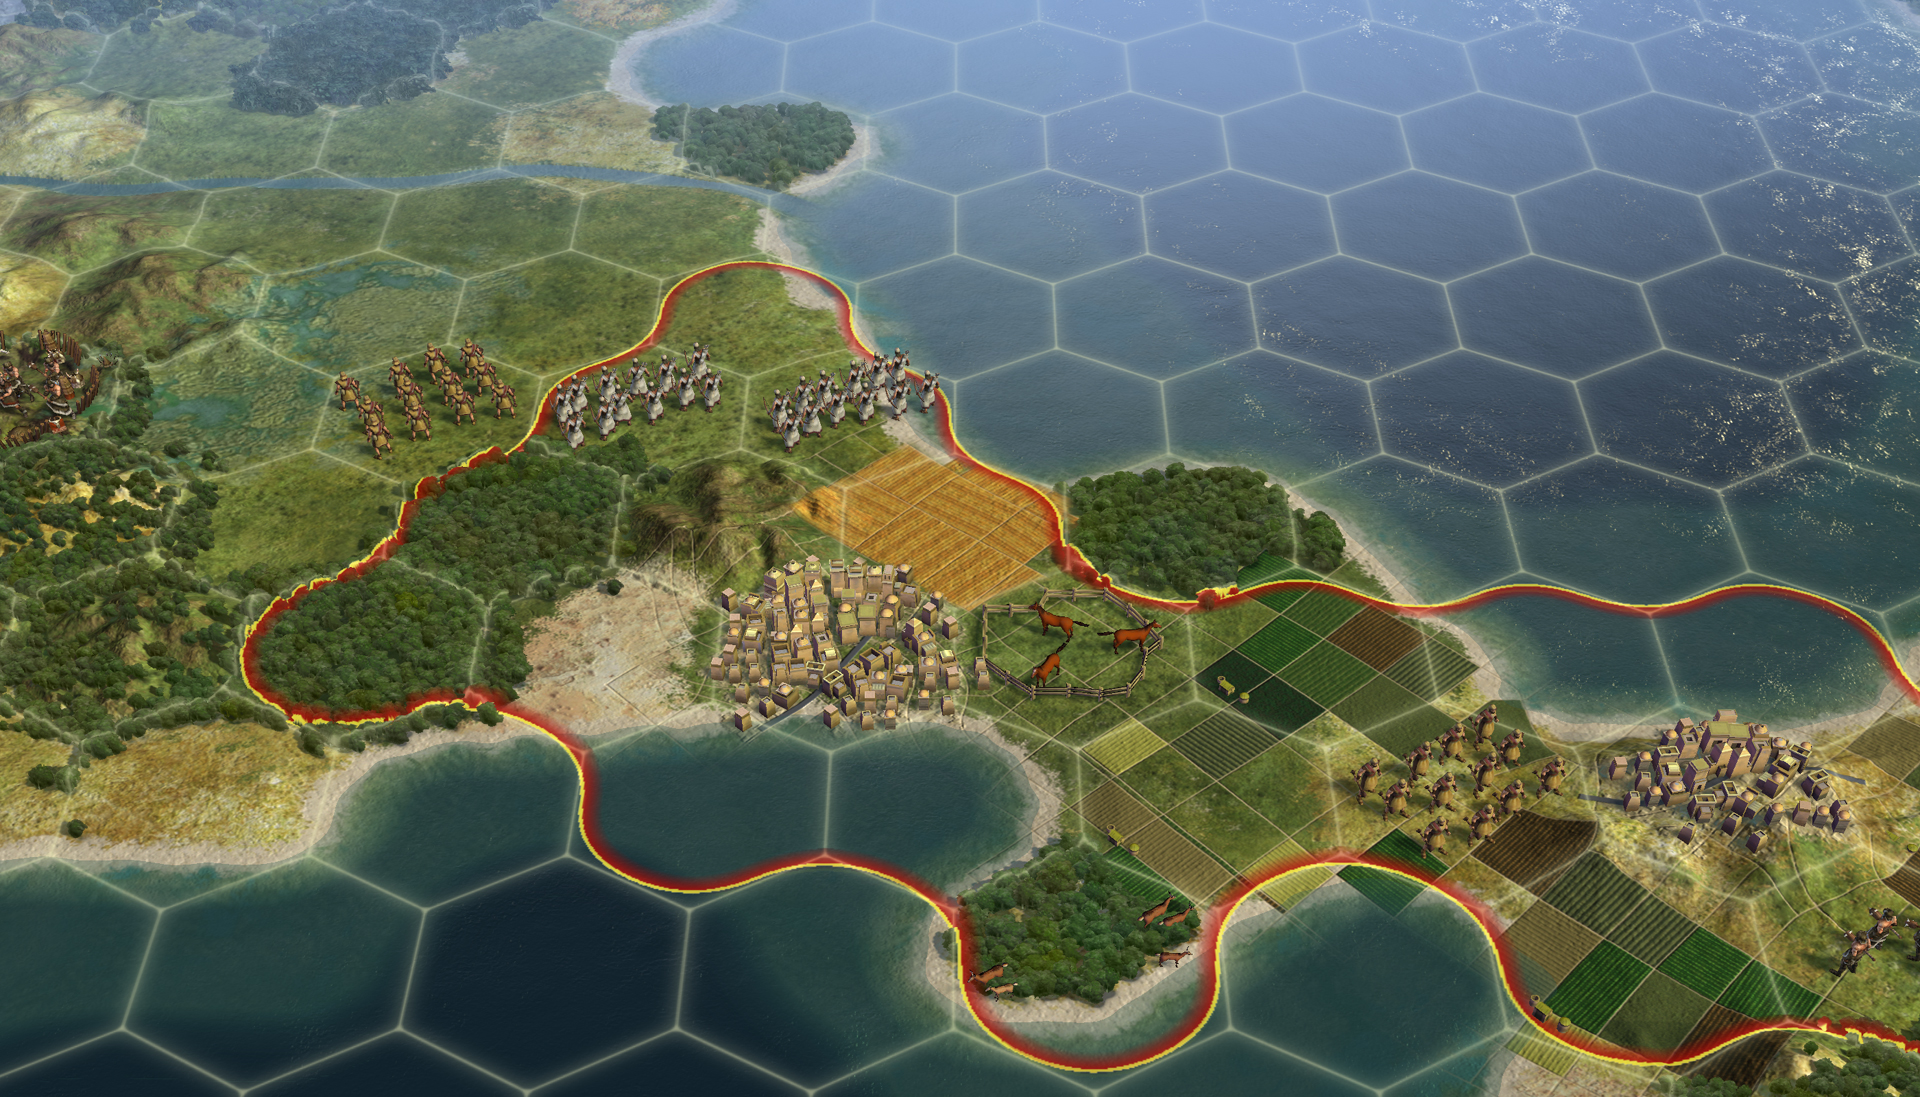
\includegraphics[trim=10cm 0cm 0cm 0cm, clip=true, height=\paperheight]{../ressources/civilization-5}\pgfsetfillopacity{1}
	}
\frame[plain]{
	\titlepage
	}
}

{
\setbeamertemplate{headline}{\vbox{\usebeamertemplate*{headlinesom}}}
\begin{frame}
	\frametitle{Sommaire}
	\tableofcontents
\end{frame} 
}



\section{Organisations guerrières}

\subsection{Armées}

\begin{frame}{Structure}
\vspace{5mm}
\begin{columns}[c]
	\begin{column}[c]{0.48\linewidth}
		\begin{centering}
		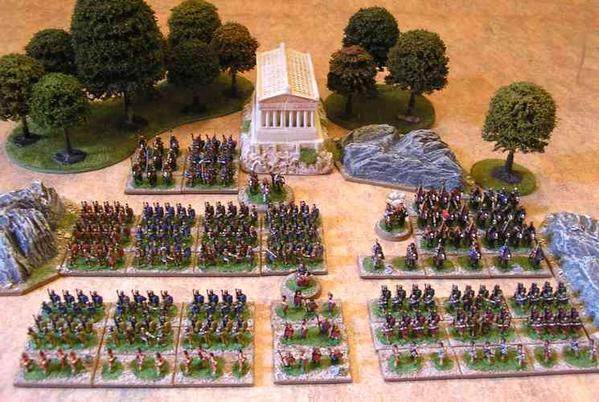
\includegraphics[width=\linewidth]{../ressources/armee_cesar}
		\end{centering}
	\end{column}
	\begin{column}[c]{0.48\linewidth}
		\begin{itemize}
			\item leader
			\begin{itemize}
				\item politique
				\item religieux
			\end{itemize}
		\end{itemize}
		\begin{itemize}
			\item homogénéité
			\begin{itemize}
				\item hiérarchie militaire
				\item formations
			\end{itemize}
		\end{itemize}
	\end{column}
\end{columns}

\bigskip
\makebox[0.99\linewidth]{
\resizebox{\paperwidth}{!}{
\begin{tabular}{| c l | c l | c l | c l |}
	\hline
	\multicolumn{8}{| c |}{\textbf{Armée}}
	\\
	\multicolumn{2}{| c |}{\textbf{Spartiate}} 	& \multicolumn{2}{ c |}{\textbf{Romaine}} & \multicolumn{2}{ c |}{\textbf{Perse}}	& \multicolumn{2}{ c |}{\textbf{Mongole}} 	\\
	\hline
	 					&			& 					&			& 				&			& \textit{Ordu}		& > 10000			\\
	 \itshape Mora 			& 576		& \itshape Légion		& 6000		& \textit{Baivarabam}& 10000		& \textit{Tumen} 	& 10000			\\
	 \itshape Loche			& 144		& \itshape Cohorte		& 600		& \textit{Hazarabam}	& 1000		& \textit{Minghan}  	& 1000			\\
	 \itshape Pentécostye	& 72			& \itshape Manipule		& 200		& \textit{satabam}	& 100		& \textit{Zuut} 		& 100			\\
	 \itshape Énomotie		& 36			& \itshape Centurie		& 100		& \textit{Dathabam} 	& 10			& \textit{Arav} 		& 10				\\
	\hline
\end{tabular}
}}
\footlineextra{\cite{mongol_army, spart_army, roman_legion,persian_army,armee_de_cesar}}
\end{frame}

\begin{frame}{Contexte}
\begin{tikzpicture}[remember picture,overlay]
	\node[anchor=north west,inner sep=0pt] at ($(current page.north west)+(0.1cm,-1.7cm)$) {
		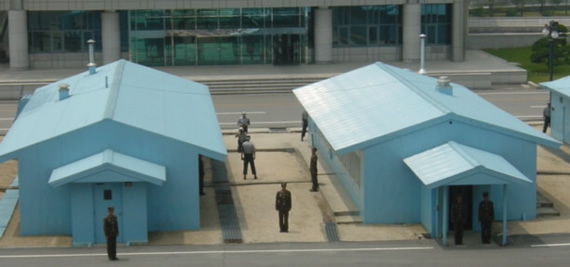
\includegraphics[height=0.38\paperheight]{../ressources/dmz-corea}
	};
	\node[anchor=south east,inner sep=0pt] at ($(current page.south east)+(-0.1cm,0.45cm)$) {
		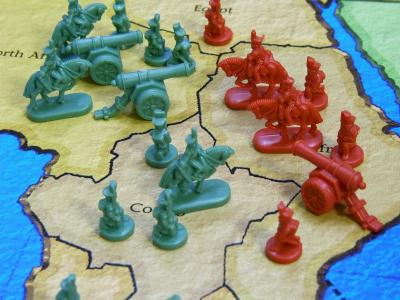
\includegraphics[height=0.38\paperheight]{../ressources/risk-board-game}
	};
	\node[anchor=north east,draw,item] at($(current page.north east)+(-1.65cm,-3.2cm)$) {défendre la patrie};
	\node[anchor=north west,draw,item] (S) at($(current page.north west)+(3.85cm,-7.0cm)$) {conquérir du territoire};
\end{tikzpicture}
\footlineextra{\cite{dmz_corea,risk_picture}}
\end{frame}


\subsection{Guérillas}

\begin{frame}{Structure}
\begin{columns}[c]
	\begin{column}[c]{0.6\linewidth}
		\begin{centering}
		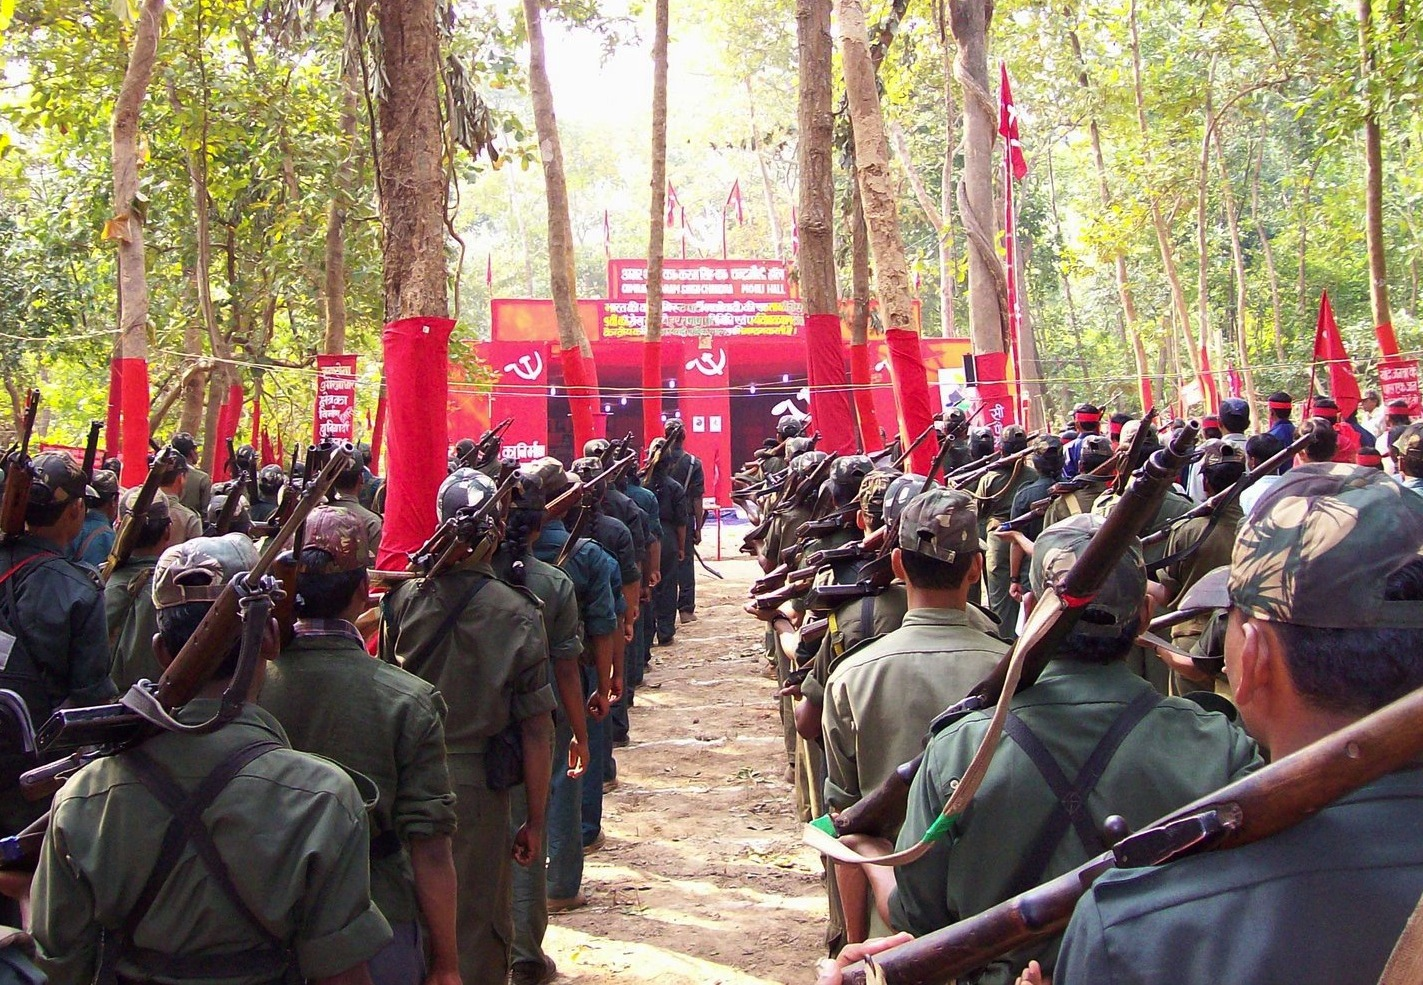
\includegraphics[width=\linewidth]{../ressources/guerrilla_naxalite}
		\end{centering}
	\end{column}
	\begin{column}[c]{0.38\linewidth}
		\begin{itemize}
			\item leader
			\begin{itemize}
				\item idéologique
				\item charismatique
			\end{itemize}
		\end{itemize}
		\begin{itemize}
			\item hétérogénéité
			\begin{itemize}
				\item hiérarchie
				\item micro-formations
			\end{itemize}
		\end{itemize}
	\end{column}
\end{columns}
\vfill
\makebox[0.99\linewidth]{
\begin{tabular}{| l | c | c | c | c |}
	\hline
	\textbf{Localisation}		& \textbf{Irlande} 	& \textbf{Inde} 	& \textbf{Cuba}	& \textbf{Colombie}	\\
	\hline
	\textbf{Régime}			& 55.000			& 1.414.000	& 35.000		& 300.000			\\
	\textbf{Insurgés}		& 15.000			& 15.000		& 200		& 20.000			\\
	\hline
\end{tabular}}
\footlineextra{\cite{guerrilla_naxalite, naxalite_guerrilla_wiki, irish_civil_war_wiki}}
\end{frame}

\begin{frame}{Contexte}
\begin{tikzpicture}[remember picture,overlay]
	\node[anchor=north west,inner sep=0pt] at ($(current page.north west)+(0.1cm,-1.7cm)$) {
	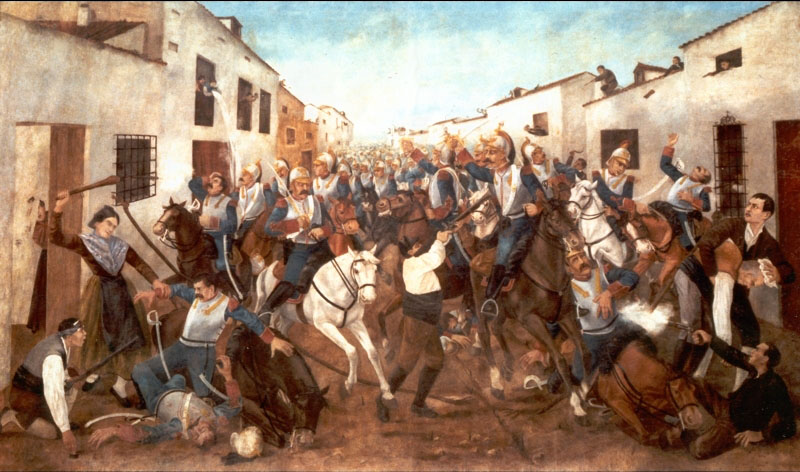
\includegraphics[height=0.4\paperheight]{../ressources/valdepenas}
	};
	\node[anchor=south west,inner sep=0pt] at ($(current page.south west)+(3.1cm,1.5cm)$) {
	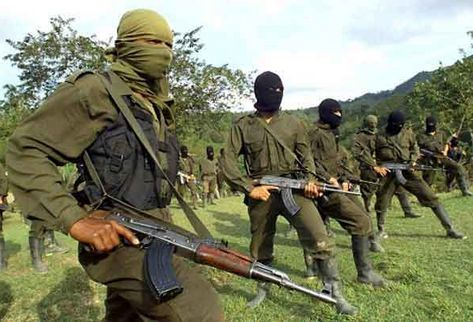
\includegraphics[height=0.4\paperheight]{../ressources/guerrilla_colombia}
	};
	\node[anchor=south east,inner sep=0pt] at ($(current page.south east)+(-2.1cm,0.45cm)$) {
	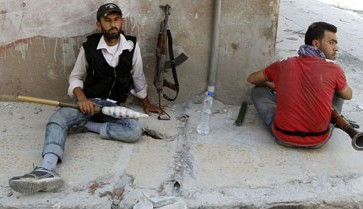
\includegraphics[trim=0cm 1.5cm 0cm 0cm, clip=true, height=0.25\paperheight]{../ressources/rebel_syrie}
	};
	\node[anchor=north east,draw,item] at($(current page.north east)+(-0.4cm,-3.0cm)$) {adaptés au terrain};
	\node[anchor=north east,draw,item] (S) at($(current page.north east)+(-0.4cm,-5.5cm)$) {mobiles};
	\node[anchor=north east,draw,item] (T) at($(current page.north east)+(-0.4cm,-7.5cm)$) {civils};
\end{tikzpicture}
\footlineextra{\cite{valdepenas,guerrilla_colombia,rebel_syrie}}
\end{frame}


\section{Stratégies militaires}

\subsection{Définitions}

\begin{frame}
\begin{tikzpicture}
\node[draw,item] (P) at(0,6) {Politique};
\node[draw=none] (Pe) at(6,6) {\begin{quote}“La politique de la guerre c’est tout simplement décider où, quand, comment, avec quels alliés et pourquoi entrer en guerre.”\end{quote}};
\end{tikzpicture}
\pause
\begin{tikzpicture}
\node[draw,item] (S) at(0,3) {Stratégie};
\node[draw=none] (Se) at(6,3) {\begin{quote}“La stratégie militaire est l'art de coordonner -au plus haut niveau de décision- l'action de l'ensemble des forces militaires de la Nation pour conduire une guerre, gérer une crise ou préserver la paix.”\end{quote}};
\end{tikzpicture}
\pause
\begin{tikzpicture}
\node[draw,item] (T) at(0,0) {Tactique};
\node[draw=none] (Te) at(6,0) {\begin{quote}“La tactique est l'art de diriger une bataille, en combinant, par la manœuvre, l'action des différents moyens de combat en vue d'obtenir le maximum d'efficacité.”\end{quote}};
\end{tikzpicture}%
\footlineextra{\cite{military_strategy, tactic, politique_jomini}}
\end{frame}

\begin{frame}
\pgfdeclareimage[width=6cm]{politique}{../ressources/alliances_ww1}
\pgfdeclareimage[width=7.5cm]{strategie}{../ressources/strategy_ww1}
\pgfdeclareimage[width=5cm]{tactique}{../ressources/Battles_of_Charleroi_ww1}
{\centering
\makebox[0pt]{%
\begin{tikzpicture}
\node[] (Si) at(0,-3) {\pgfbox[left,center] {\pgfuseimage{strategie}}};
\node[] (Pi) at(12.6,-2.66) {\pgfbox[right,bottom] {\pgfuseimage{politique}}};
\node[] (Ti) at(12.6,-5.7) {\pgfbox[right,center] {\pgfuseimage{tactique}}};
\node[draw,item] (P) at(5.5,0.4) {Politique};
\node[draw,item] (S) at(8.5,-3.2) {Stratégie};
\node[draw,item] (T) at(5.5,-6.5) {Tactique};
\end{tikzpicture}%
}\par
}
\footlineextra{\cite{ww1, military_strategy, tactic}}
\end{frame}


\subsection{Stratégies}

\begin{frame}
\frametitle{Sun Tzu}
\framesubtitle{Chine (\siecle{6} BC)}
\begin{tikzpicture}[remember picture,overlay]
	\node[anchor=north east,inner sep=0pt] at ($(current page.north east)+(-0.1cm,-0.75cm)$) {
	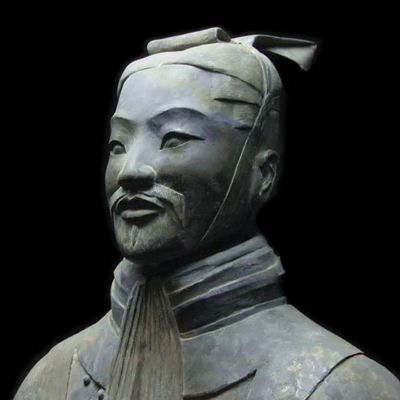
\includegraphics[width=1.9cm]{../ressources/sun_tzu_general}
  };
\end{tikzpicture}
\begin{quote}“L'art de la guerre, c'est de soumettre l'ennemi sans combat.”\end{quote}
\vfill
\begin{columns}[t]
\begin{column}{0.5\linewidth}
Préceptes
\begin{itemize}
\item prendre toutes les possessions de l'adversaire et les conserver intactes
\item adaptabilité, préparation, connaissance du terrain et des forces en présence (espionnage)
\end{itemize}
\end{column}
\begin{column}{0.5\linewidth}
Axes stratégiques
\begin{enumerate}
\item cause morale
\item conditions climatiques
\item conditions géographiques
\item qualités du dirigeant
\item organisation et discipline
\end{enumerate}
\end{column}
\end{columns}

\footlineextra{\cite{tzu1997art, sun_tzu_fighting, sun_tzu_wiki}}
\end{frame}

\begin{frame}{Alexandre le grand}
\framesubtitle{Grèce (\siecle{4} BC)}
\begin{tikzpicture}[remember picture,overlay]
	\node[anchor=north east,inner sep=0pt] at ($(current page.north east)+(-0.1cm,-0.75cm)$) {
	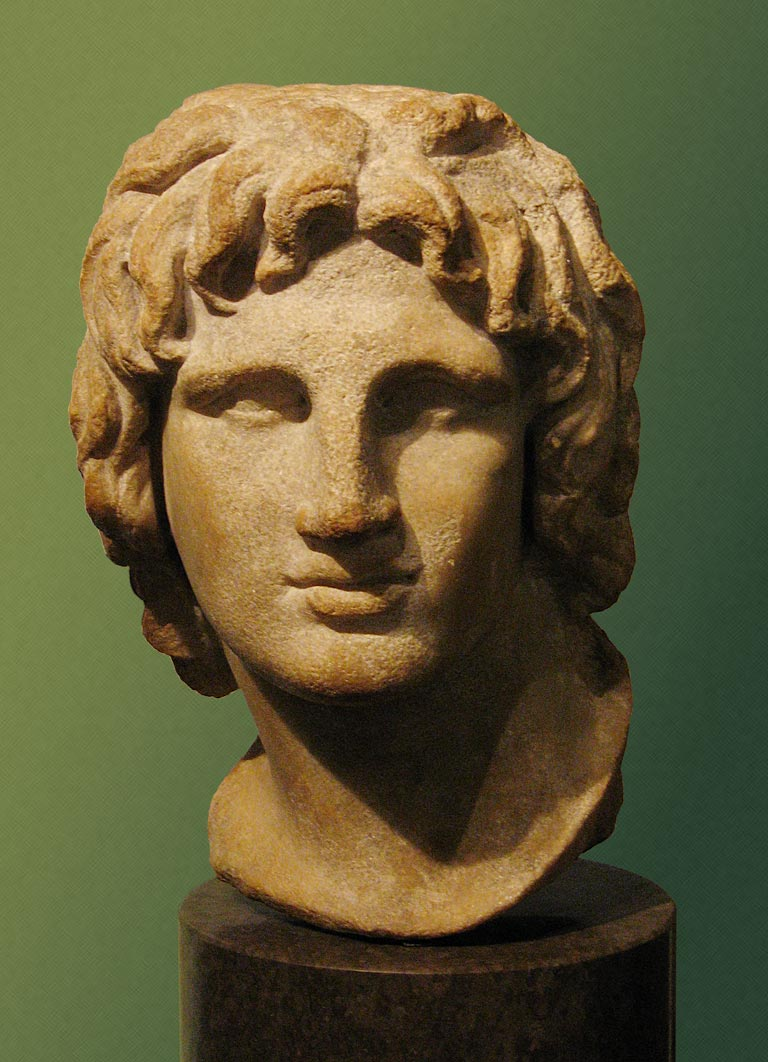
\includegraphics[trim=0cm 8cm 0cm 0cm, clip=true, width=1.9cm]{../ressources/AlexanderTheGreat_Bust}
  };
\end{tikzpicture}
\begin{quote}“Ce qui ne me tue pas me rend plus fort.”\end{quote}
\vfill
\begin{columns}[t]
\begin{column}{0.5\linewidth}
Préceptes
\begin{itemize}
\item conscription et intégration des peuples vaincus
\item allègement de l'équipement des troupes
\end{itemize}
\end{column}
\begin{column}{0.5\linewidth}
Axes stratégiques
\begin{enumerate}
\item assurer ses arrières
\item choisir judicieusement la voie d'accès pour chaque conquête
\end{enumerate}
\end{column}
\end{columns}
\footlineextra{\cite{alexander_the_great, alexandre_balkans}}
\end{frame}

\begin{frame}{Julius Caesar}
\framesubtitle{Italie (\siecle{1} BC)}
\begin{tikzpicture}[remember picture,overlay]
	\node[anchor=north east,inner sep=0pt] at ($(current page.north east)+(-0.1cm,-0.75cm)$) {
	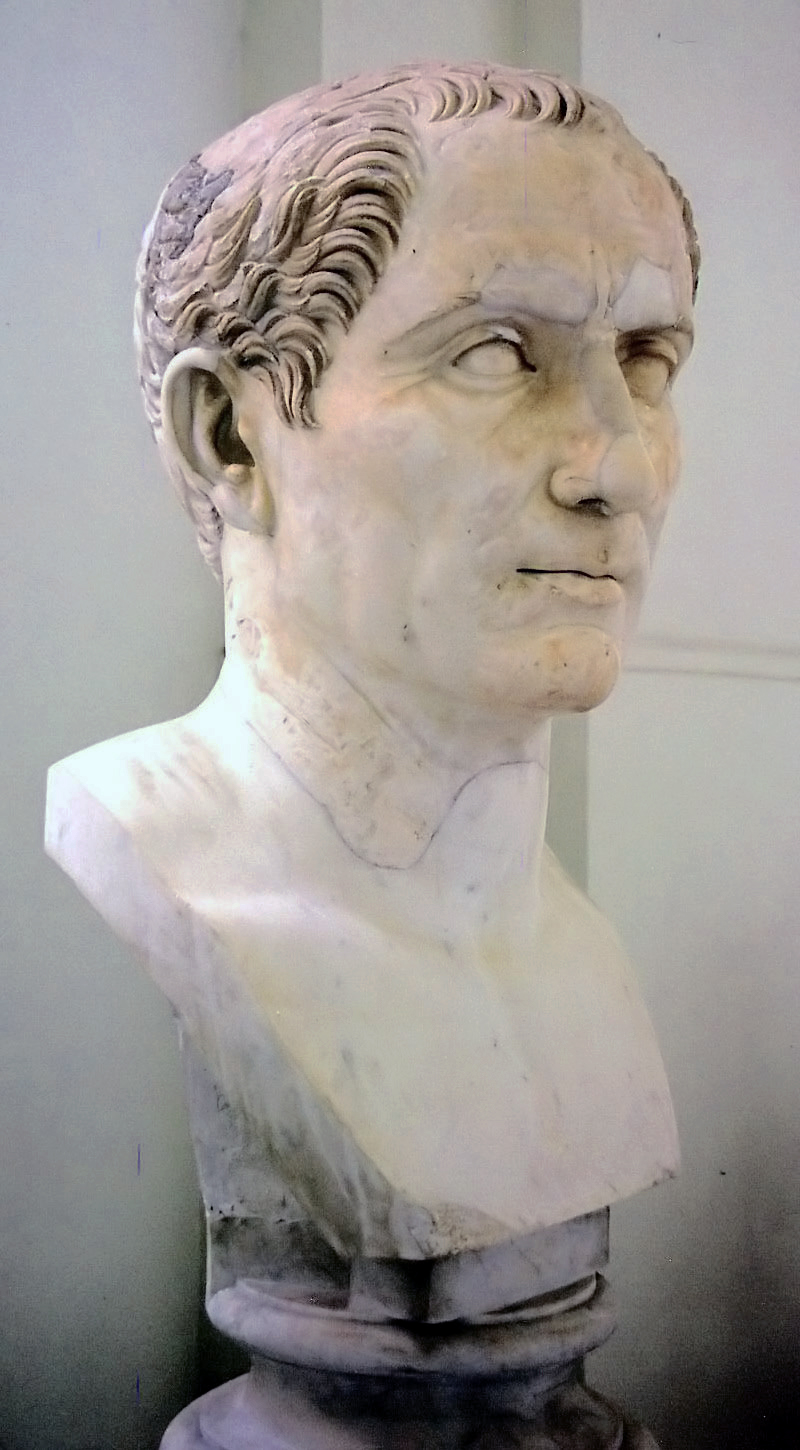
\includegraphics[trim=0cm 20cm 0cm 0cm, clip=true, width=1.9cm]{../ressources/cesare}
  };
\end{tikzpicture}
\begin{quote}“L’expérience, voilà le maître en toutes choses.”\end{quote}
\vfill
\begin{columns}[t]
\begin{column}{0.5\linewidth}
Préceptes
\begin{itemize}
\item stabilité militaire et logistique
\end{itemize}
\end{column}
\begin{column}{0.5\linewidth}
Axes stratégiques
\begin{enumerate}
\item infanterie lourde
\item bataillons étrangers spécialisés
\item formations en fonction des conditions géographiques
\item bivouac fortifié
\end{enumerate}
\end{column}
\end{columns}
\footlineextra{\cite{caesar_wiki, caesar_lacks}}
\end{frame}

\begin{frame}{Genghis Khan}
\framesubtitle{Mongolie (\siecle{12})}
\begin{tikzpicture}[remember picture,overlay]
	\node[anchor=north east,inner sep=0pt] at ($(current page.north east)+(-0.1cm,-0.75cm)$) {
	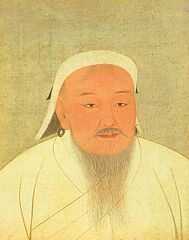
\includegraphics[trim=0cm 1cm 0cm 1cm, clip=true, width=1.9cm]{../ressources/genghis_khan}
  };
\end{tikzpicture}
\begin{quote}“Le plus grand bonheur du Mongol est de vaincre l’ennemi, de ravir ses trésors, de faire hurler ses serviteurs, de se sauver au galop de ses chevaux bien nourris [\ldots]”\end{quote}
\vfill
\begin{columns}[t]
\begin{column}{0.5\linewidth}
Préceptes
\begin{itemize}
\item guerre psychologique
\item règne de la terreur
\item connaissance du terrain : espionnage ; éclaireurs
\end{itemize}
\end{column}
\begin{column}{0.5\linewidth}
Axes stratégiques
\begin{enumerate}
\item peu de troupes ; avant-garde forte
\item troupes montées % logistique et vitesse
\item délégation des décisions
\item relais de communication et ravitaillement
\item attaques biologiques
\end{enumerate}
\end{column}
\end{columns}
\footlineextra{\cite{khan_wiki, military_strategy, mongol_army}}
\end{frame}

\begin{frame}{Napoléon Bonaparte}
\framesubtitle{France (\siecle{18})}
\begin{tikzpicture}[remember picture,overlay]
	\node[anchor=north east,inner sep=0pt] at ($(current page.north east)+(-0.1cm,-0.75cm)$) {
	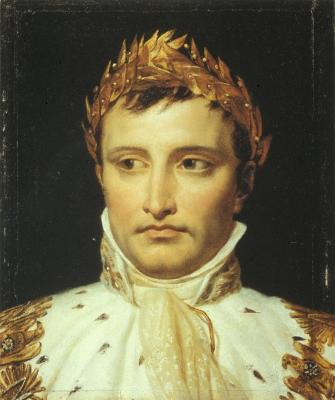
\includegraphics[trim=0cm 2cm 0cm 0cm, clip=true, width=1.9cm]{../ressources/napoleon}
  };
\end{tikzpicture}
\begin{quote}“Réunir ses feux contre un seul point ; une fois la brèche faite, l’équilibre est rompu, tout le reste devient inutile.”\end{quote}
\vfill
\begin{columns}[t]
\begin{column}{0.5\linewidth}
Préceptes
\begin{itemize}
\item recherche systématique de la bataille
\item destruction totale des forces adverses
\item être le plus fort à l’endroit où l’on a décidé de frapper le coup décisif
\end{itemize}
\end{column}
\begin{column}{0.5\linewidth}
Axes stratégiques
\begin{enumerate}
\item vitesse de manœuvre : {\emph Blitzkrieg}
\item fortifications
\item lignes de réapprovisionnement provisoires
\item artillerie
\end{enumerate}
\end{column}
\end{columns}
\footlineextra{\cite{napoleon, napoleon_wiki, napoleon_portrait}}
\end{frame}

\begin{frame}{~ }
\begin{tabular}{|p{0.45\linewidth}|p{0.45\linewidth}|}
\hline
\emph{Stratégie indirecte} & \emph{Stratégie directe}\\
\hline
renseignement & conscription\\
embuscade & recherche de la bataille décisive\\
tromperie & planification et formations\\
sabotage & fortifications\\
\hline
\end{tabular}
\begin{tikzpicture}[remember picture,overlay]
	\node[anchor=south east,inner sep=0pt] at ($(current page.south east)+(-1.35cm,0.4cm)$) {
		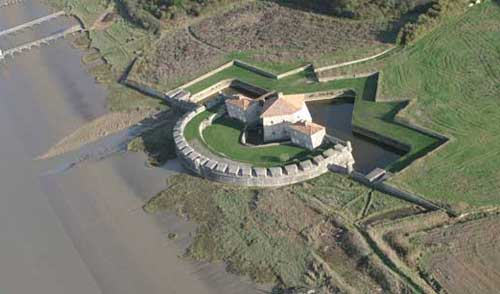
\includegraphics[trim=1.5cm 0cm 0cm 0cm, clip=true, scale=0.31]{../ressources/Vauban_Fort_Lupin}
	};
	\node[anchor=north east,inner sep=0pt] at ($(current page.north east)+(-2.4cm,-0.8cm)$) {
		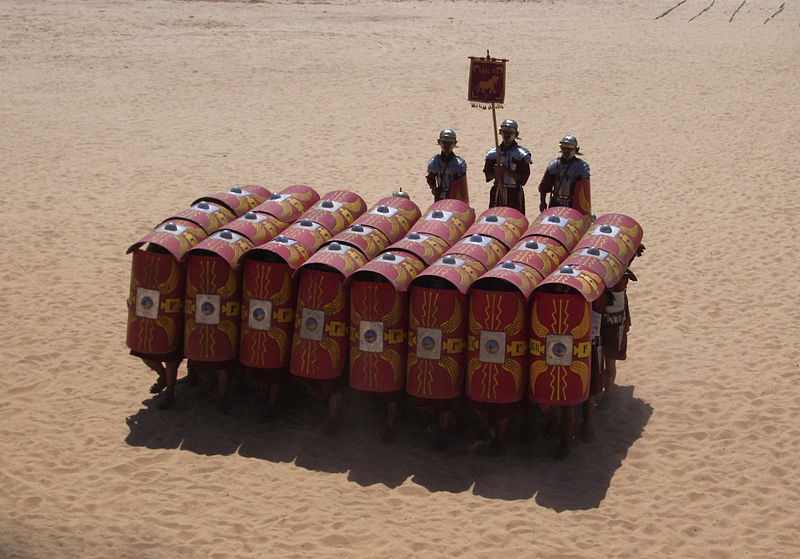
\includegraphics[trim=0cm 1cm 0cm 1cm, clip=true, scale=0.14]{../ressources/tortue}
	};
	\node[anchor=north west,inner sep=0pt] at ($(current page.north west)+(2.15cm,-0.8cm)$) {
		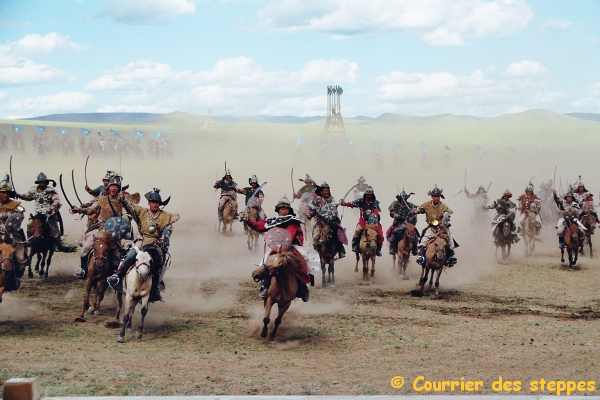
\includegraphics[trim=0cm 1cm 0cm 0cm, clip=true, scale=0.19]{../ressources/mongol_army}
	};
	\node[anchor=south west,inner sep=0pt] at ($(current page.south west)+(1.3cm,0.4cm)$) {
		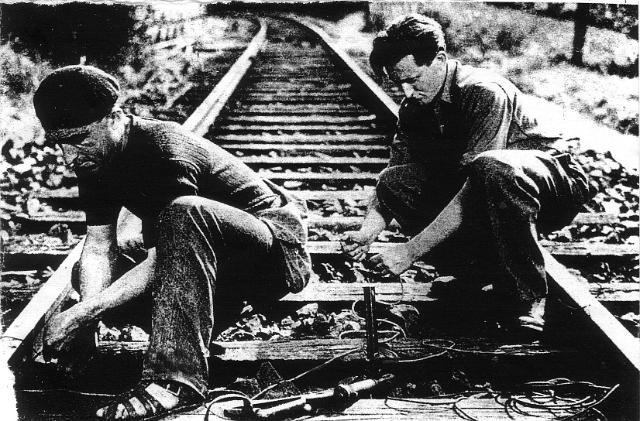
\includegraphics[scale=0.217]{../ressources/sabotage_maquisards}
	};
\end{tikzpicture}
\footlineextra{\cite{fort_lupin,war}}
\end{frame}


\subsection{Formations et unités}

\begin{frame}{Infanterie}
\begin{tikzpicture}[remember picture,overlay]
	\node[anchor=south west,inner sep=0pt] at ($(current page.south west)+(0.1cm,0.45cm)$) {
		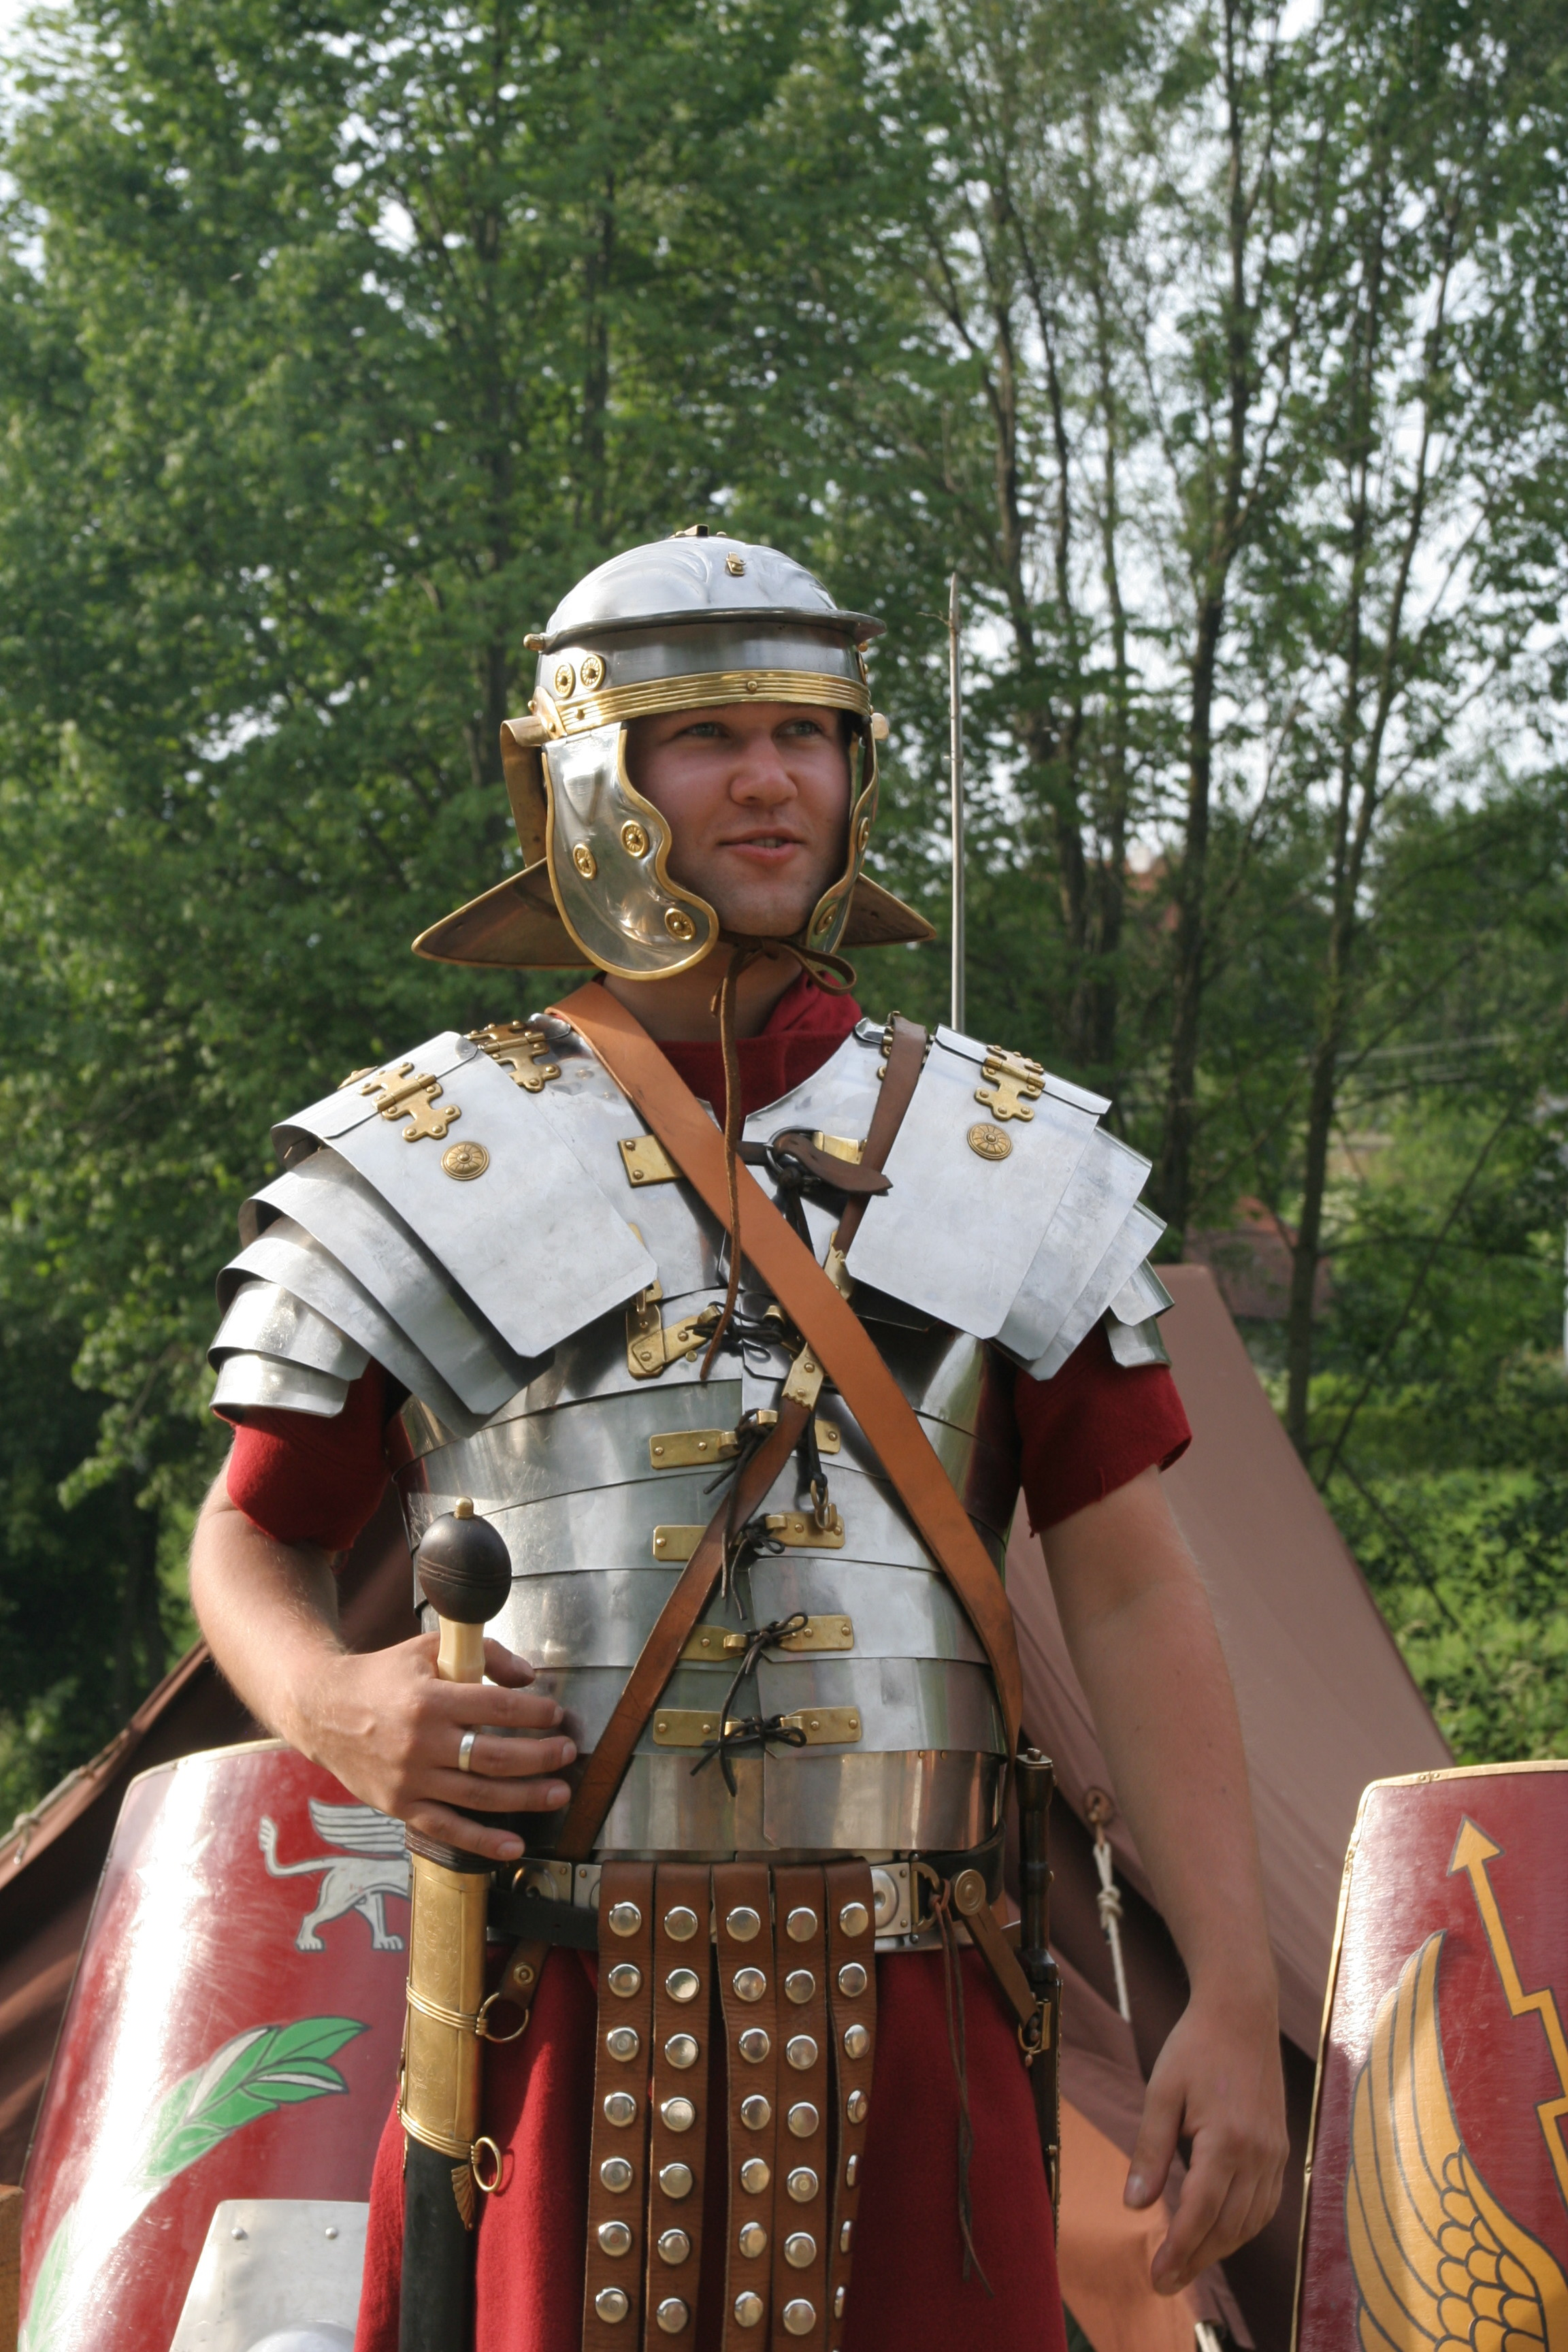
\includegraphics[trim=0cm 0cm 0cm 15cm, clip=true, width=0.42\paperwidth]{../ressources/Roman_soldier}
	};
	\node[anchor=north east,inner sep=0pt] at ($(current page.north east)+(-0.15cm,-2.6cm)$) {
		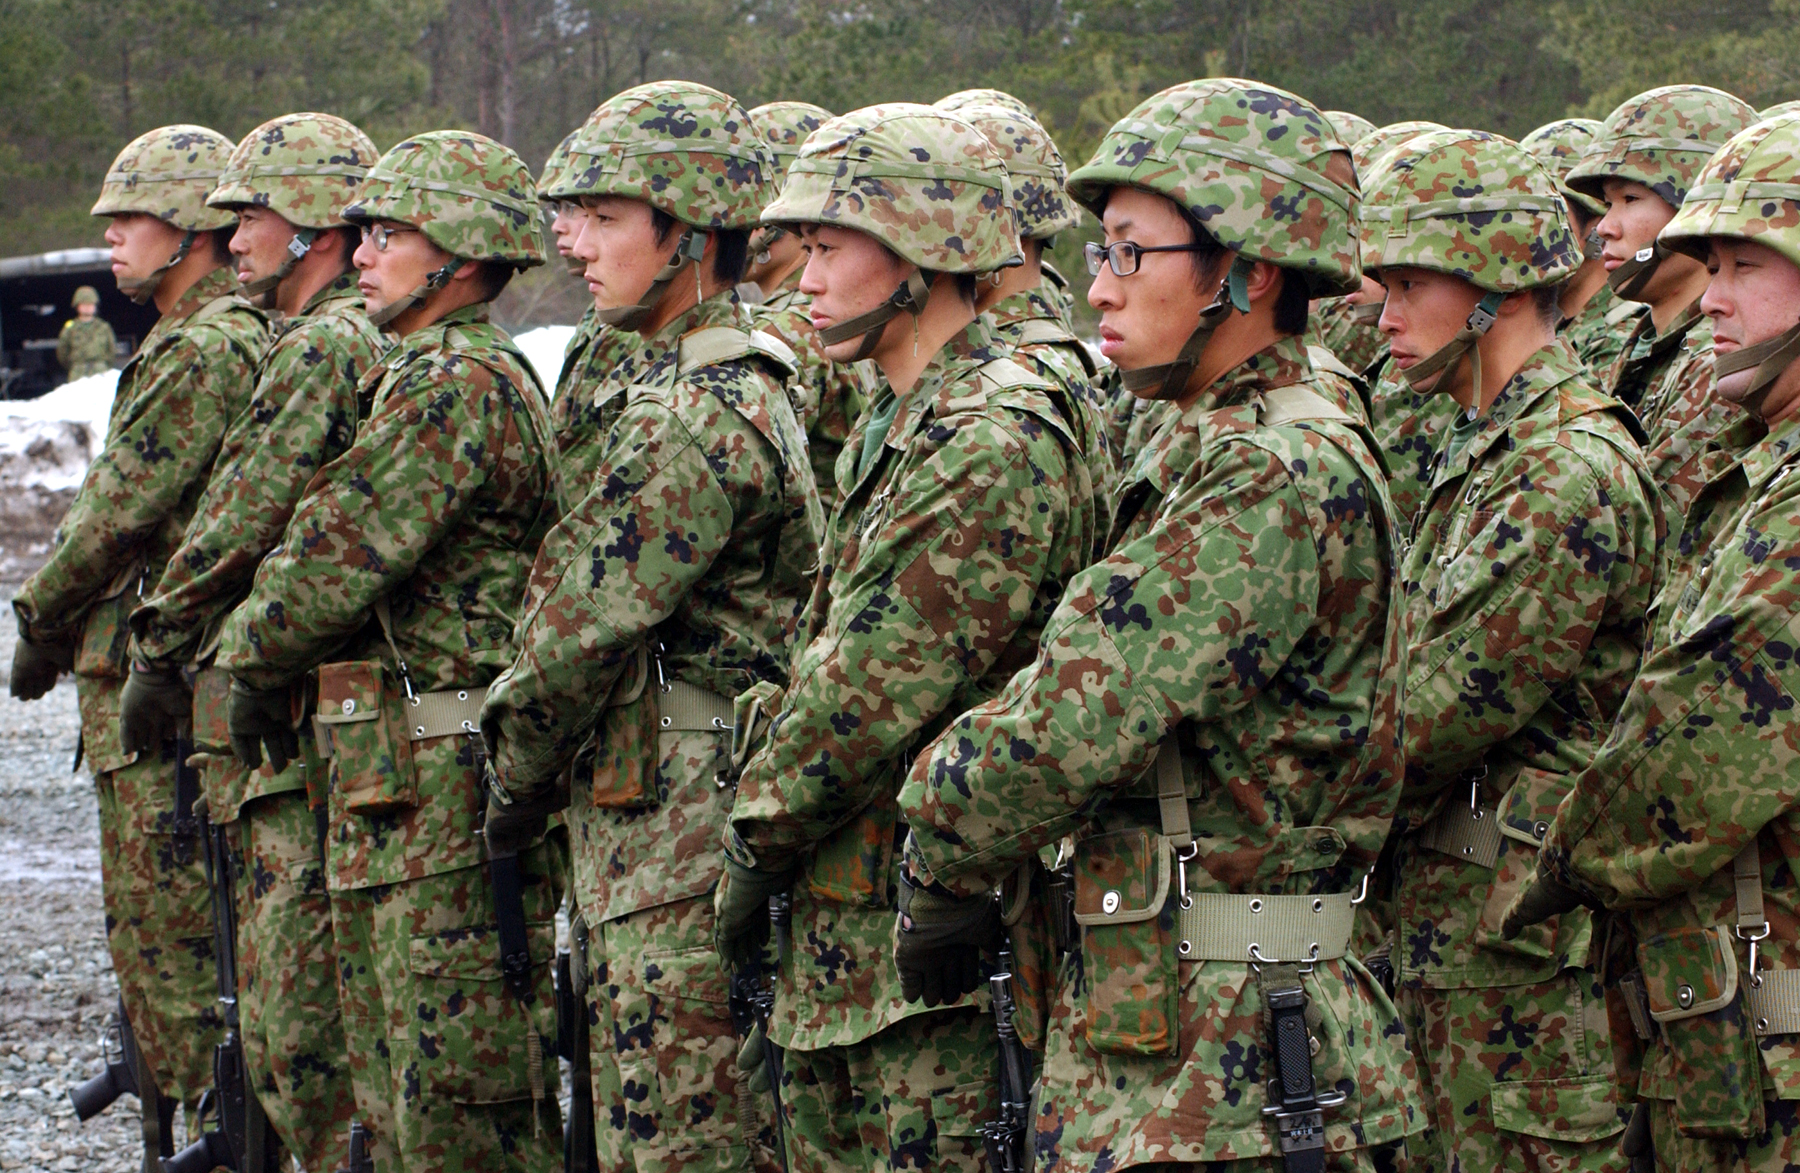
\includegraphics[width=0.55\paperwidth]{../ressources/JGDSF_Soldiers}
	};
\end{tikzpicture}
\footlineextra{\cite{infantery}}
\end{frame}

\begin{frame}{Cavalerie légère}
\begin{tikzpicture}[remember picture,overlay]
	\node[anchor=north west,inner sep=0pt] at ($(current page.north west)+(0.1cm,-2.6cm)$) {
		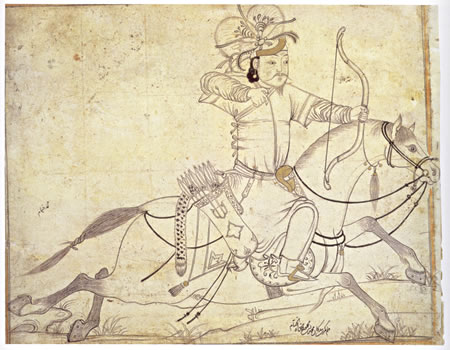
\includegraphics[width=0.5\paperwidth]{../ressources/IlkhanidHorseArcher}
	};
	\node[anchor=north east,inner sep=0pt] at ($(current page.north east)+(-0.15cm,-1.6cm)$) {
		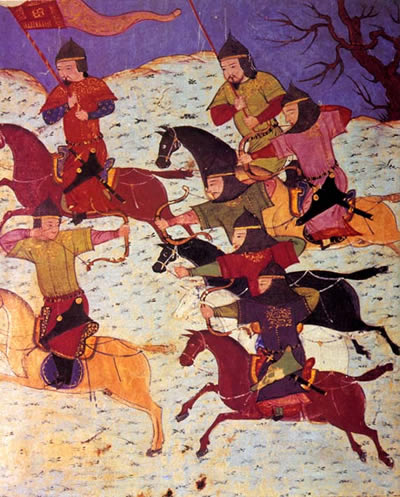
\includegraphics[width=0.47\paperwidth]{../ressources/MongolCavalrymen}
	};
\end{tikzpicture}
\footlineextra{\cite{archery,mongol_army}}
\end{frame}

\begin{frame}{Cavalerie lourde}
\begin{tikzpicture}[remember picture,overlay]
	\node[anchor=south west,inner sep=0pt] at ($(current page.south west)+(0.1cm,0.45cm)$) {
		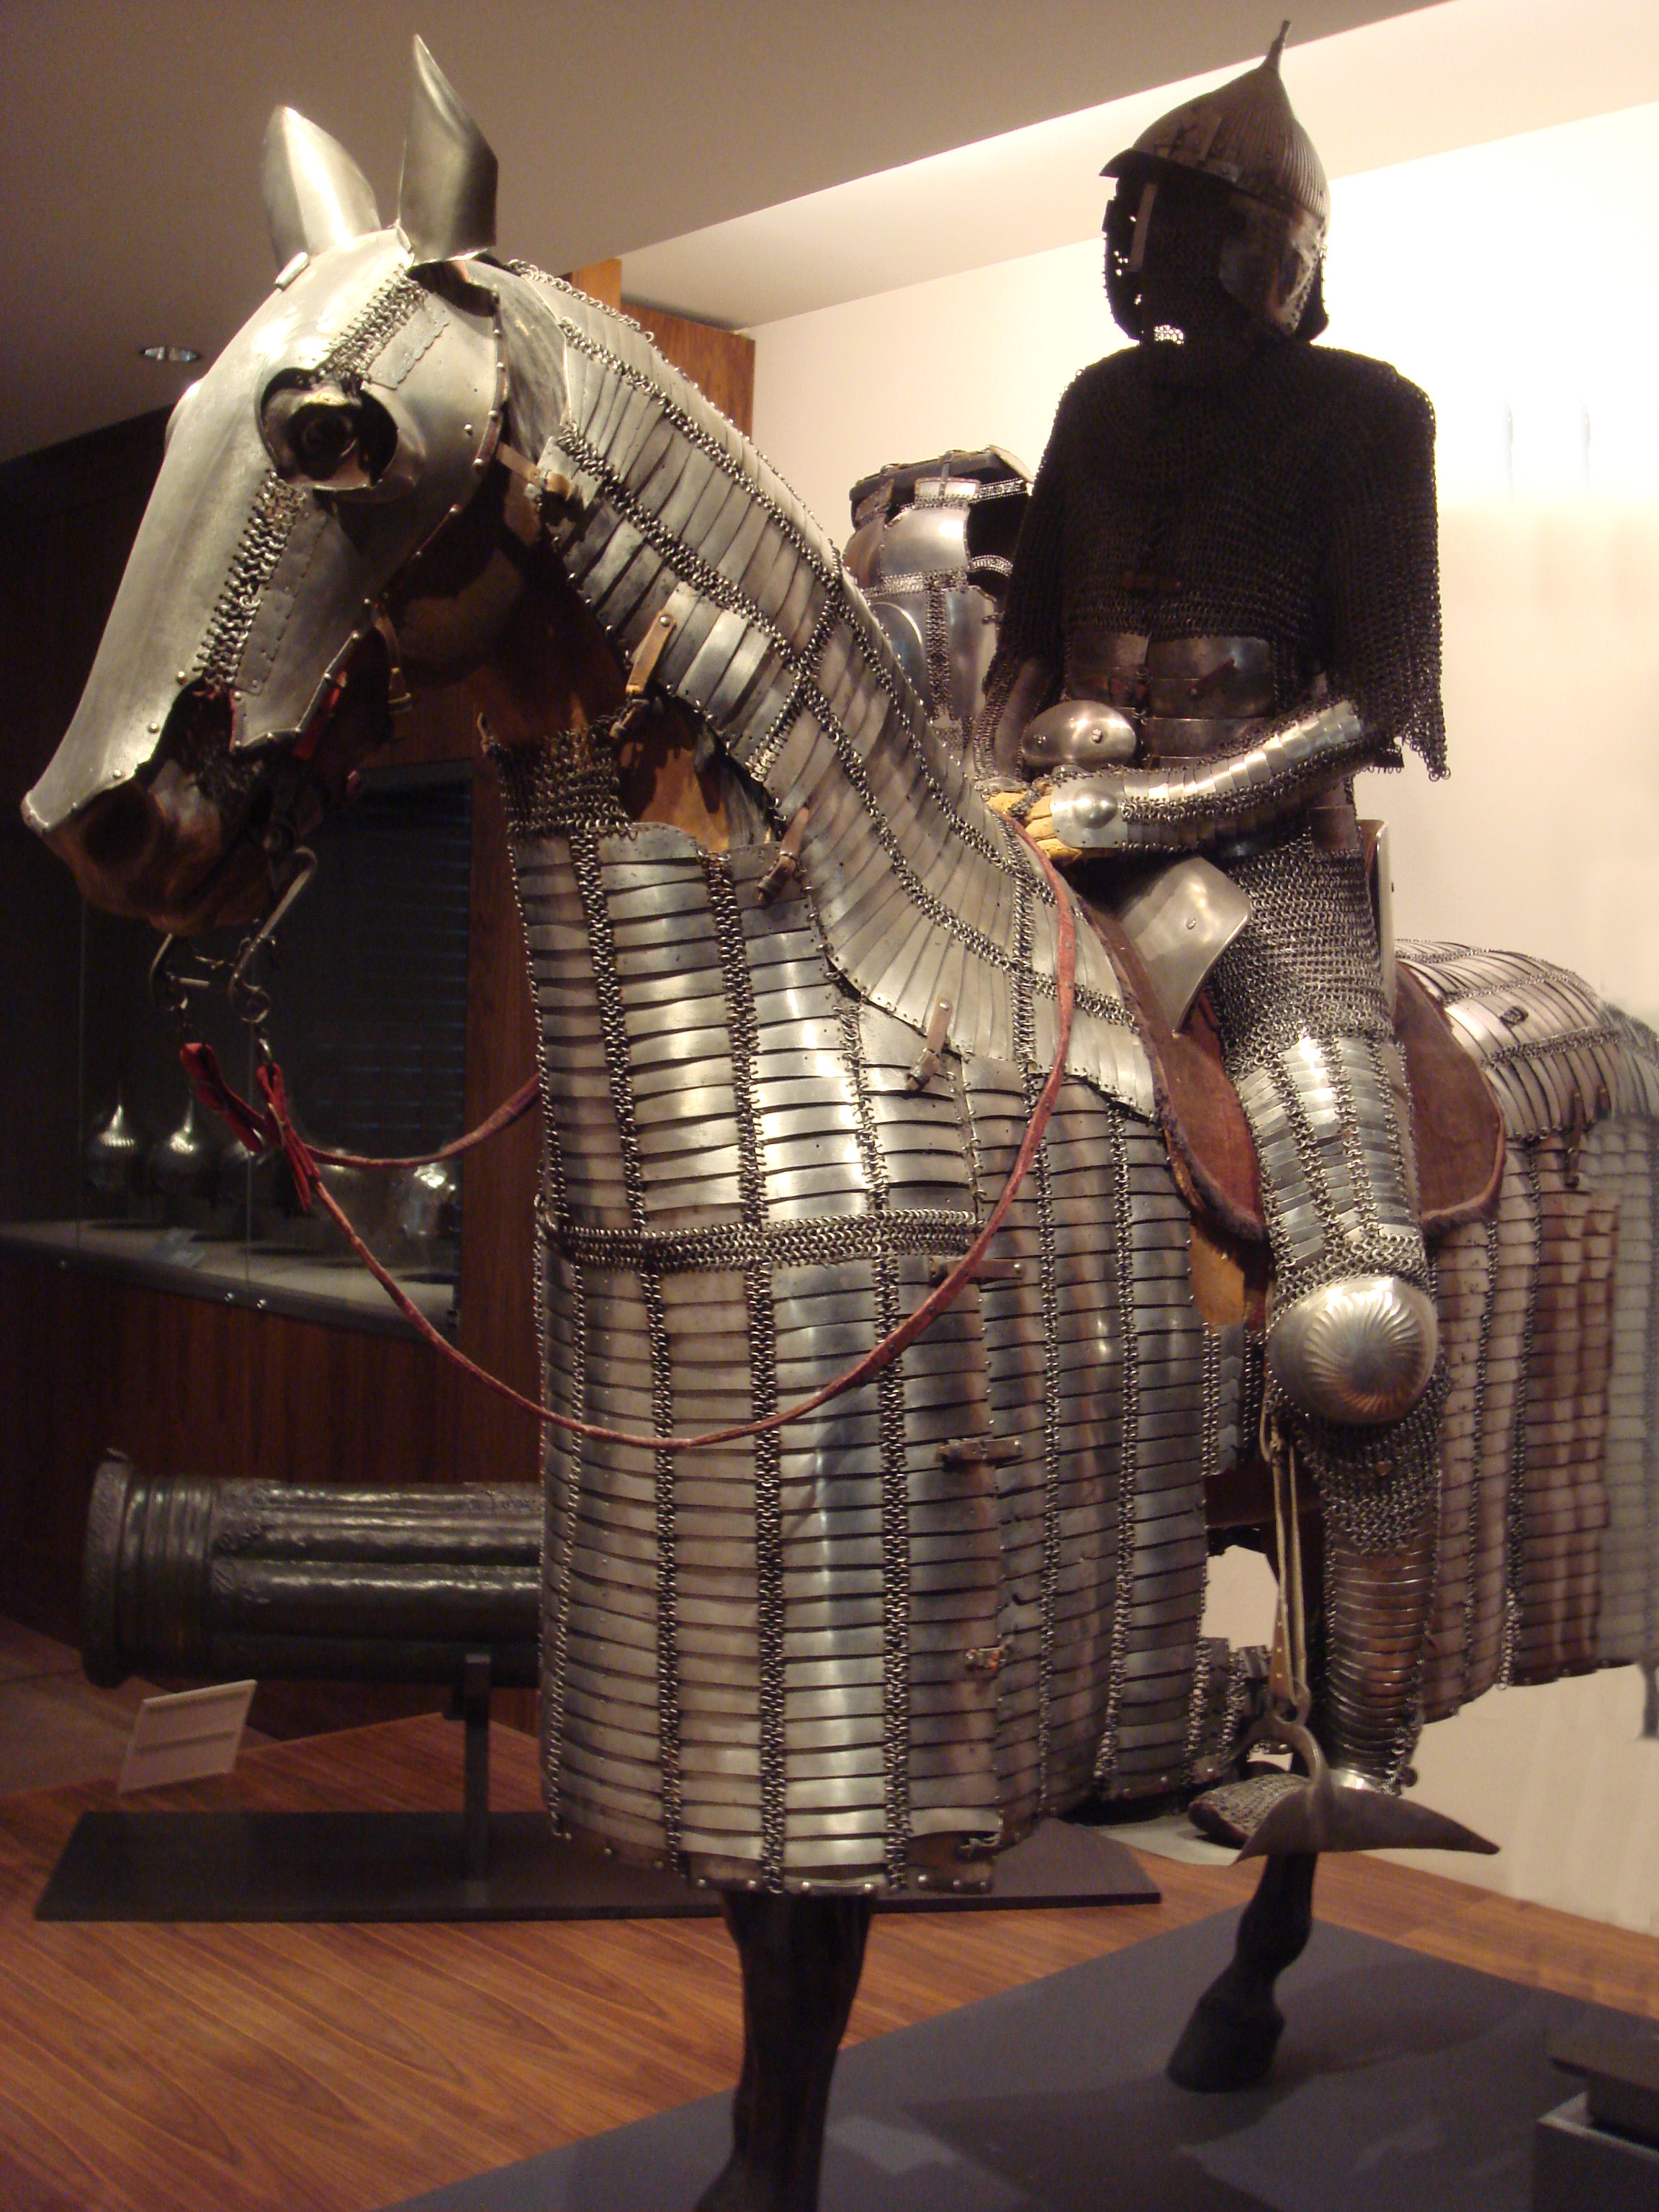
\includegraphics[width=0.44\paperwidth]{../ressources/Ottoman_Mamluk_horseman}
	};
	\node[anchor=south east,inner sep=0pt] at ($(current page.south east)+(-0.15cm,0.45cm)$) {
		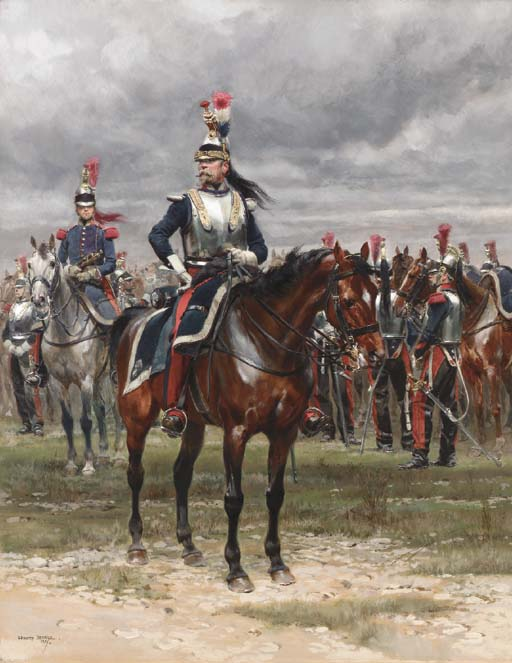
\includegraphics[width=0.5\paperwidth]{../ressources/cuirassiers}
	};
\end{tikzpicture}
\footlineextra{\cite{heavy_cavalry}}
\end{frame}

\begin{frame}{Formation en triple ligne}
\begin{tikzpicture}[remember picture,overlay]
	\node[anchor=north west,inner sep=0pt] at ($(current page.north west)+(2.5cm,-1.6cm)$) {
	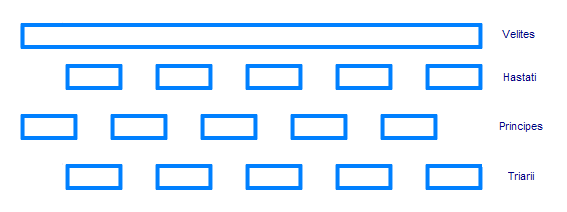
\includegraphics[scale=0.4]{../ressources/Polybian_formation}
	};
	\node[anchor=south west,inner sep=0pt] at ($(current page.south west)+(1.3cm,0.2cm)$) {
	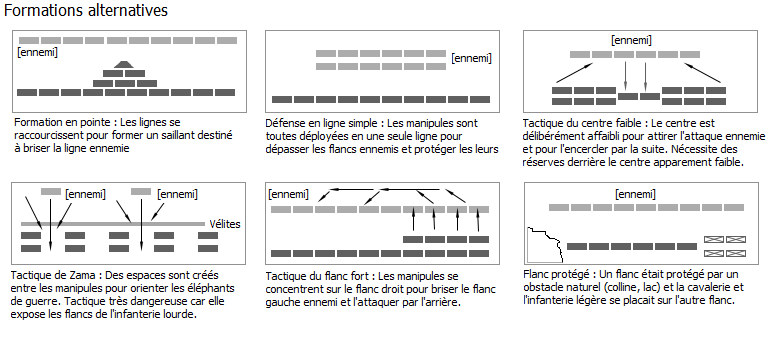
\includegraphics[scale=0.5]{../ressources/Formations_infanterie_romaine}
	};
\end{tikzpicture}
\footlineextra{\cite{roman_infantry_tactics}}
\end{frame}


\subsection{Tactiques}

\begin{frame}{Charge}
\begin{tikzpicture}[remember picture,overlay]
	\node[anchor=north east,inner sep=0pt] at ($(current page.north east)+(-0.1cm,-0.75cm)$) {
	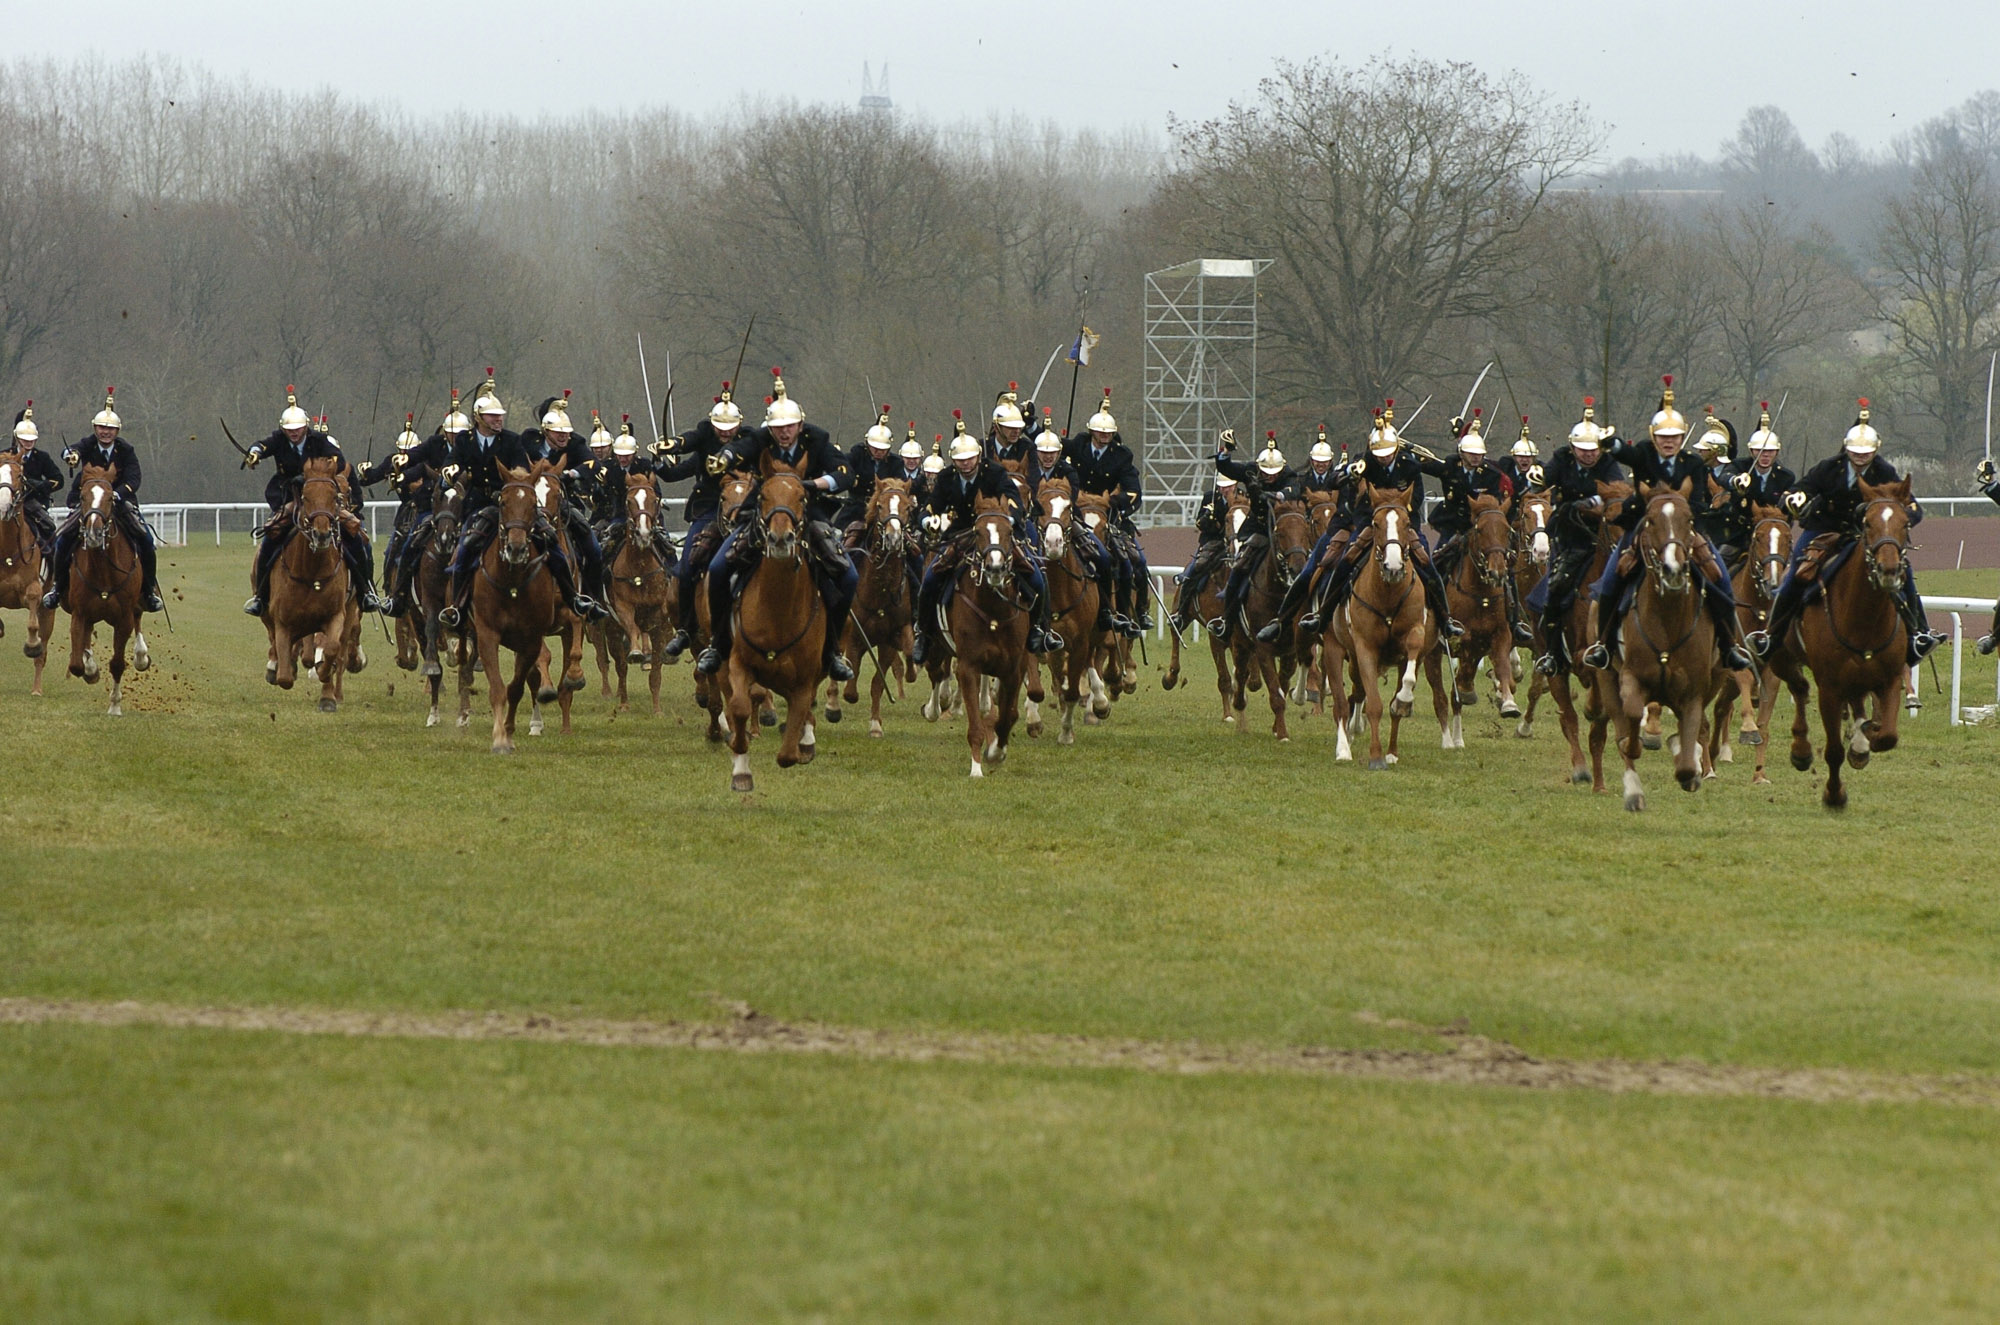
\includegraphics[height=0.5\paperheight]{../ressources/Charge-de-cavalerie}
	};
	\node[anchor=south west,inner sep=0pt] at ($(current page.south west)+(0.1cm,0.45cm)$) {
	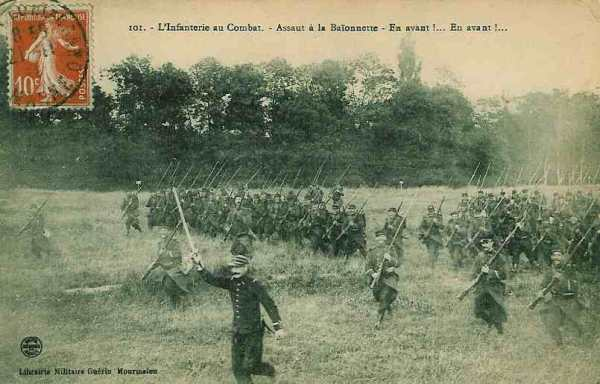
\includegraphics[height=0.53\paperheight]{../ressources/charge_infanterie}
	};
	\node[draw,item,anchor=north west] at($(current page.north west)+(0.2cm,-3.4cm)$) {infanterie};
	\node[draw,item,anchor=north east] at($(current page.north east)+(-0.2cm,-5.65cm)$) {cavalerie};
\end{tikzpicture}
\footlineextra{\cite{charge_tactic, charge_cavalery}}
\end{frame}

\begin{frame}{Manœuvre de flanquement}
\begin{tikzpicture}[remember picture,overlay]
	\node[anchor=north east,inner sep=0pt] at ($(current page.north east)+(-0.1cm,-0.75cm)$) {
	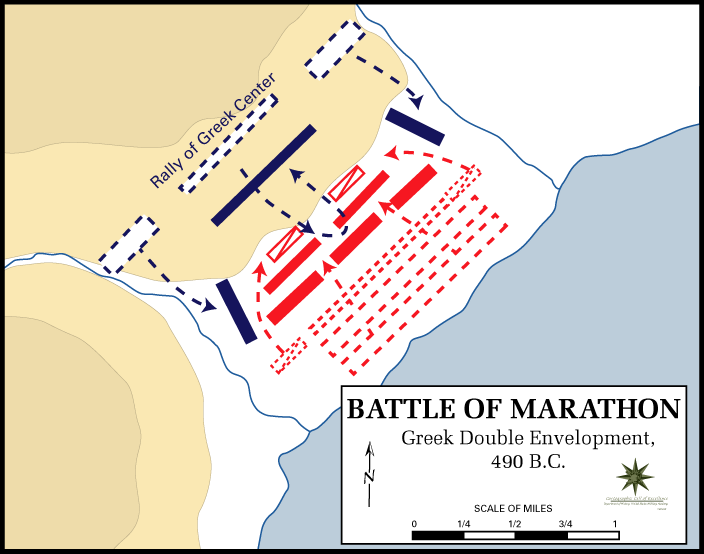
\includegraphics[height=0.5\paperheight]{../ressources/Battle_of_Marathon}
	};
	\node[anchor=south west,inner sep=0pt] at ($(current page.south west)+(0.1cm,0.45cm)$) {
	\fbox{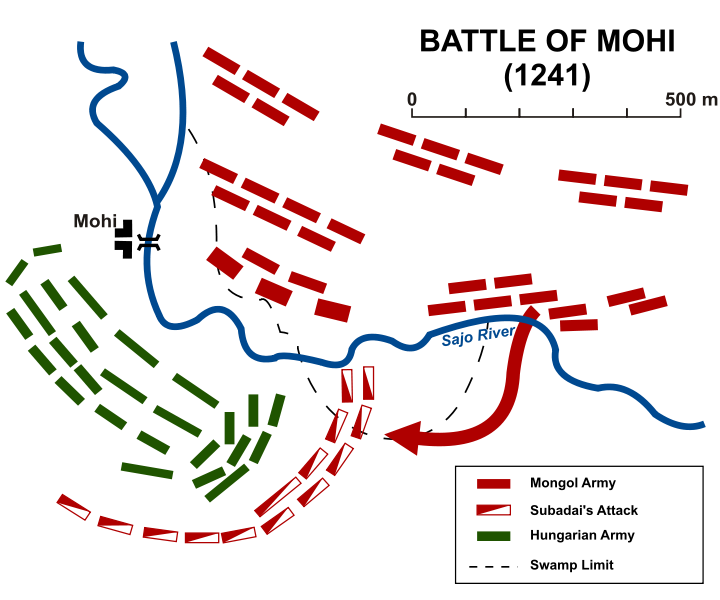
\includegraphics[height=0.53\paperheight]{../ressources/Battle_of_Mohi}}
	};
	\node[draw,item,anchor=north east] at($(current page.north east)+(-0.2cm,-5.7cm)$) {prise en tenaille};
\end{tikzpicture}
\footlineextra{\cite{tactic, flanking_maneuver, pincer_tactic}}
\end{frame}

\begin{frame}{Le marteau et l'enclume}
\begin{tikzpicture}[remember picture,overlay]
	\node[anchor=north west,inner sep=0pt] at ($(current page.north west)+(1cm,-1.75cm)$) {
	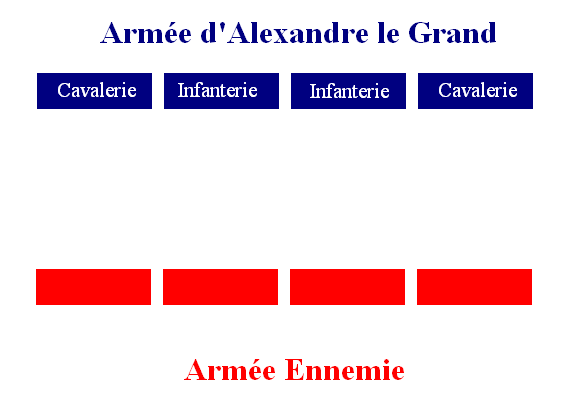
\includegraphics[trim=0.5cm 0.5cm 0.5cm 0.5cm, clip=true, scale=0.25]{../ressources/marteau}
	};
	\node[anchor=north east,inner sep=0pt] at ($(current page.north east)+(-1cm,-1.75cm)$) {
	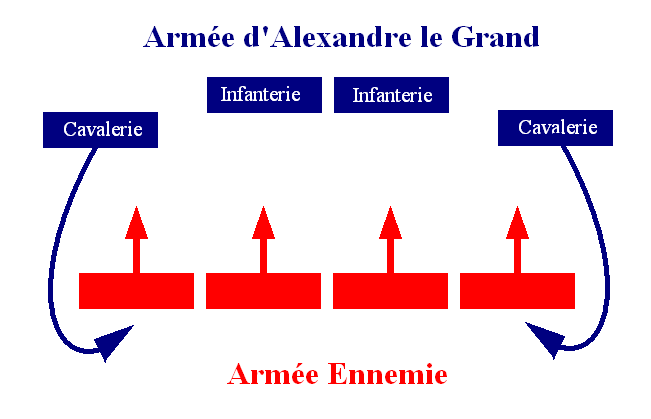
\includegraphics[trim=0.5cm 0.7cm 0.5cm 0.7cm, clip=true, scale=0.25]{../ressources/marteau2}
	};
	\node[anchor=south west,inner sep=0pt] at ($(current page.south west)+(1cm,0.45cm)$) {
	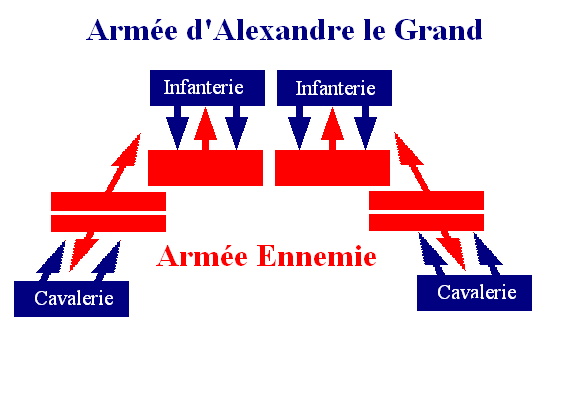
\includegraphics[scale=0.25]{../ressources/enclume}
	};
	\node[anchor=south east,inner sep=0pt] at ($(current page.south east)+(-1.4cm,1.2cm)$) {
	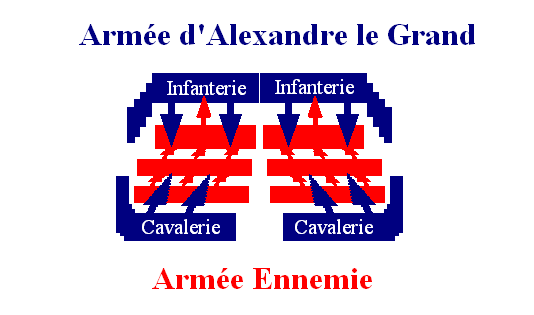
\includegraphics[scale=0.25]{../ressources/enclume2}
	};
\end{tikzpicture}
\footlineextra{\cite{Alexanders_tactics}}
\end{frame}

\begin{frame}{Contre-attaque}
\begin{tikzpicture}[remember picture,overlay]
	\node[anchor=north west,inner sep=0pt] at ($(current page.north west)+(0.1cm,-1.6cm)$) {
	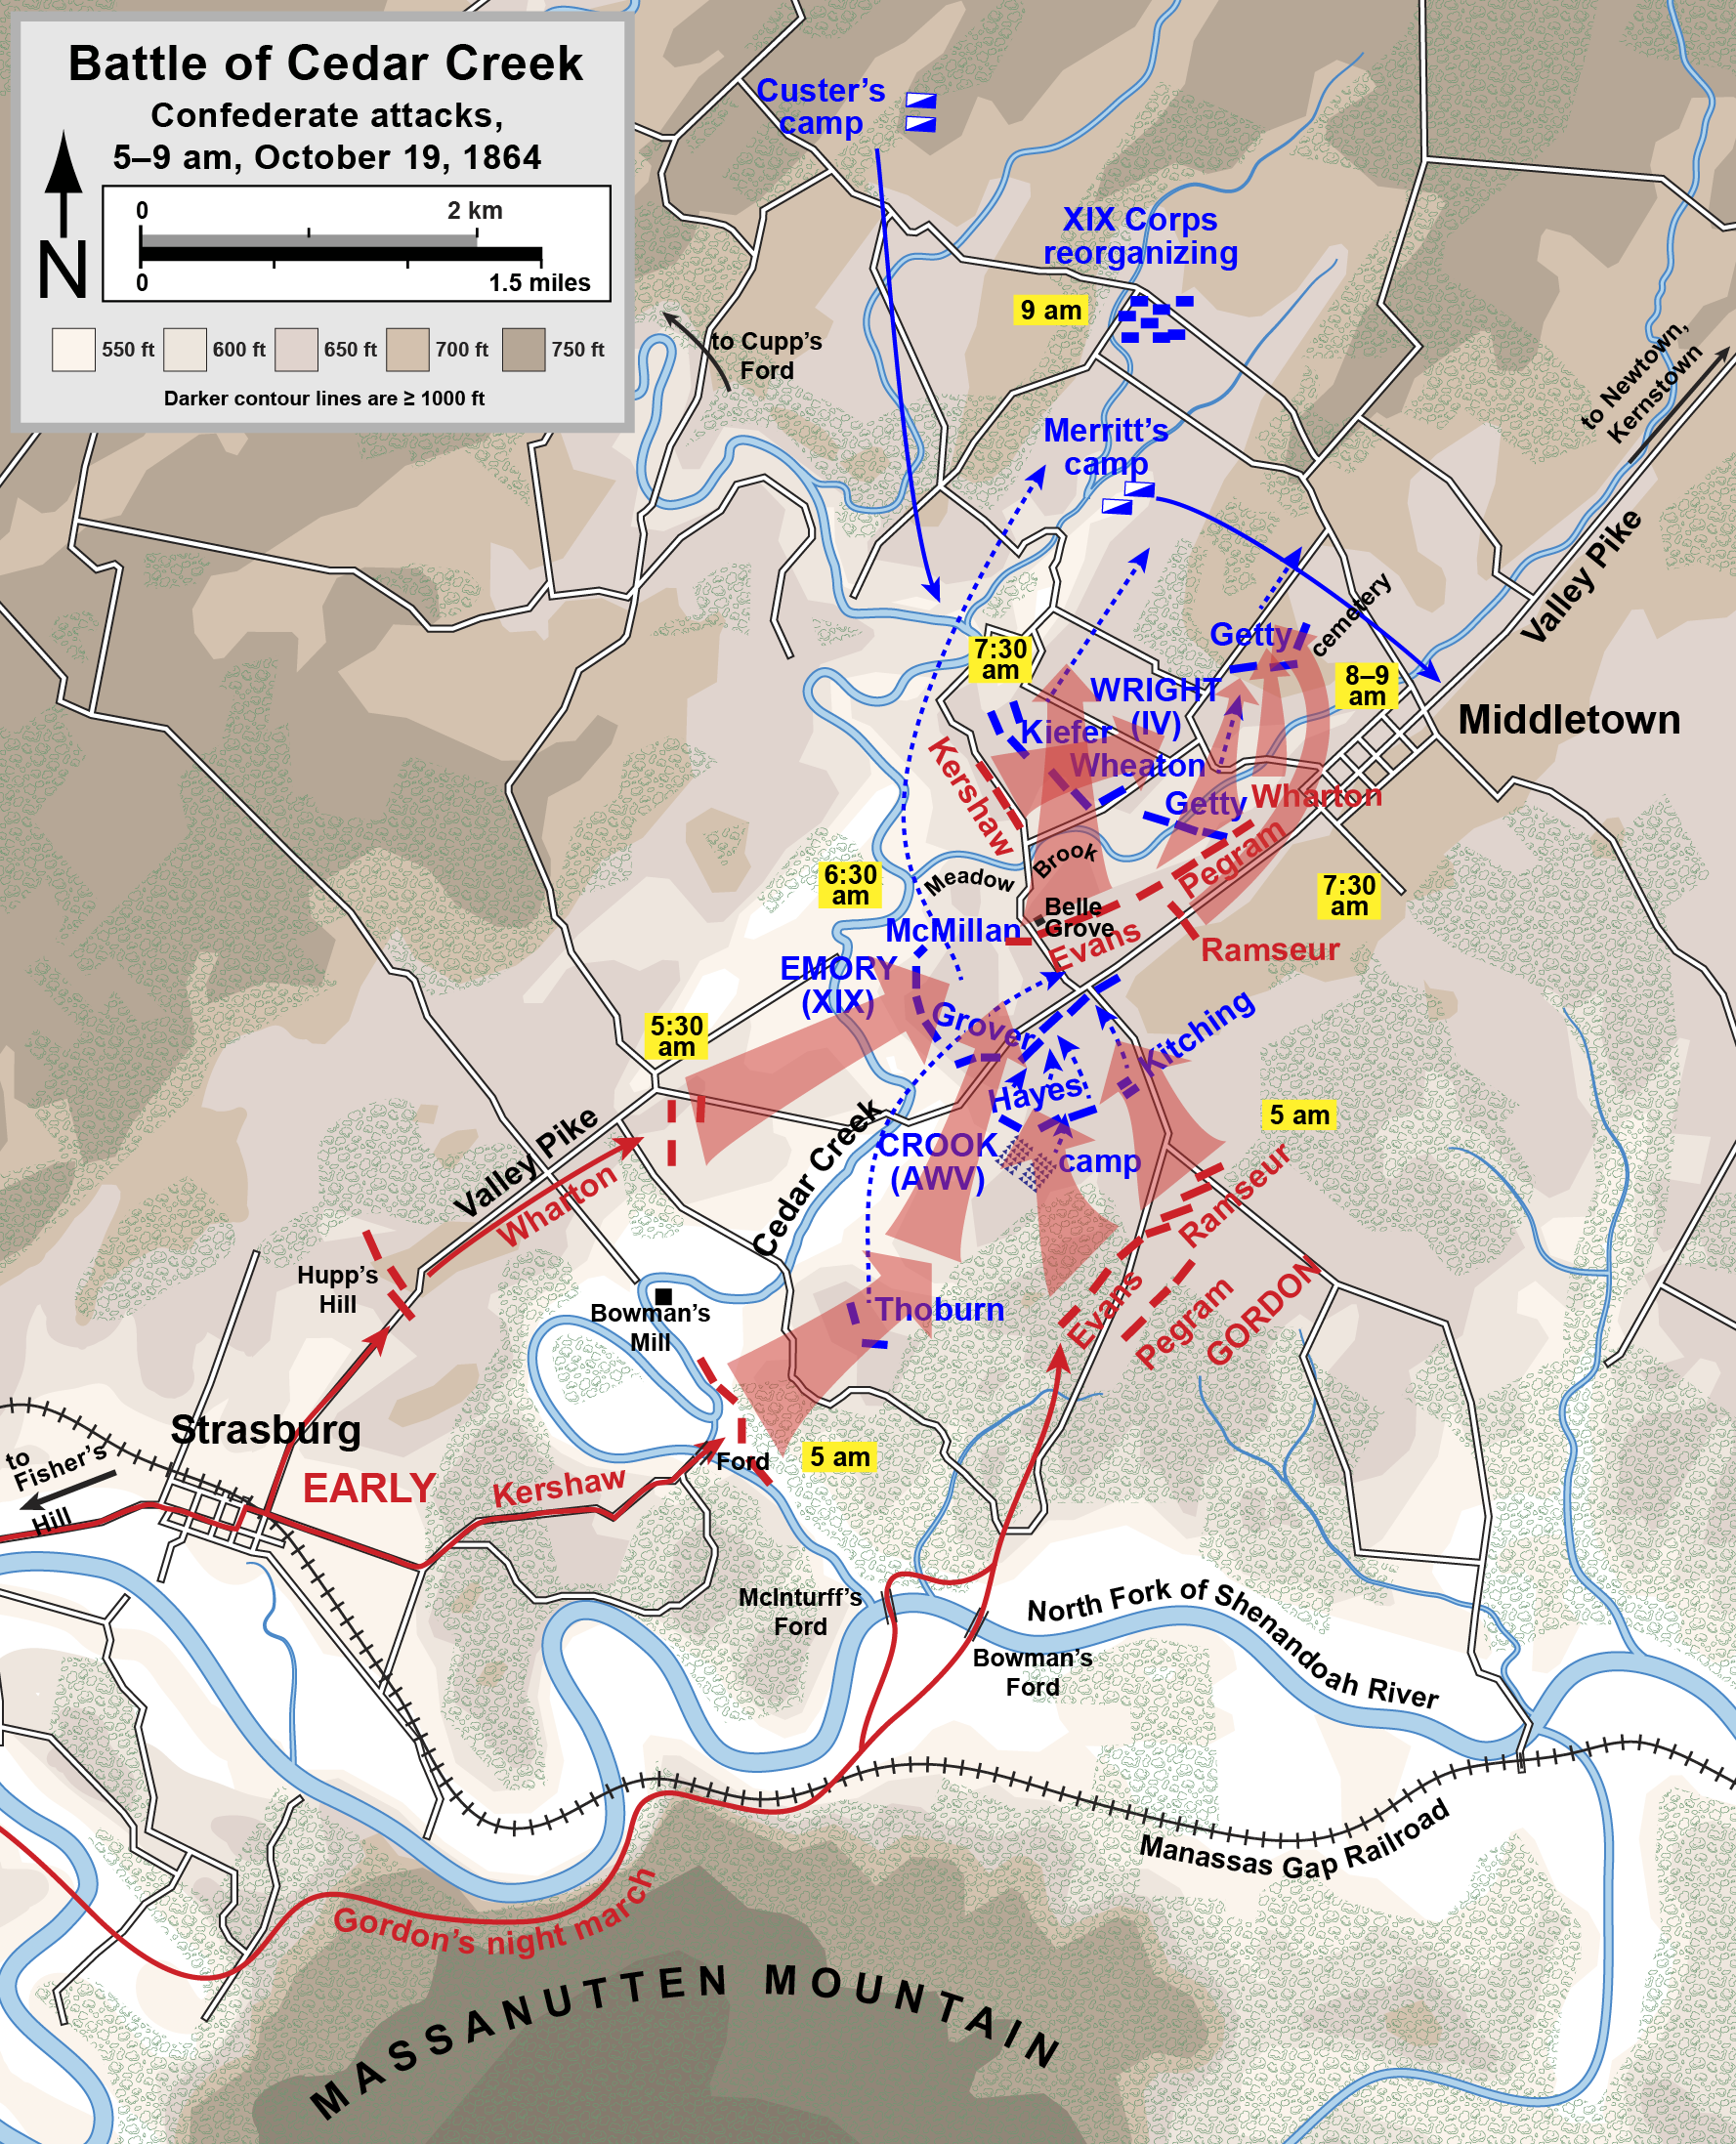
\includegraphics[trim=0cm 2.5cm 0cm 0cm, clip=true, width=0.47\paperwidth]{../ressources/Cedar_Creek_Confederate_attacks}
	};
	\node[anchor=north east,inner sep=0pt] at ($(current page.north east)+(-0.15cm,-1.6cm)$) {
	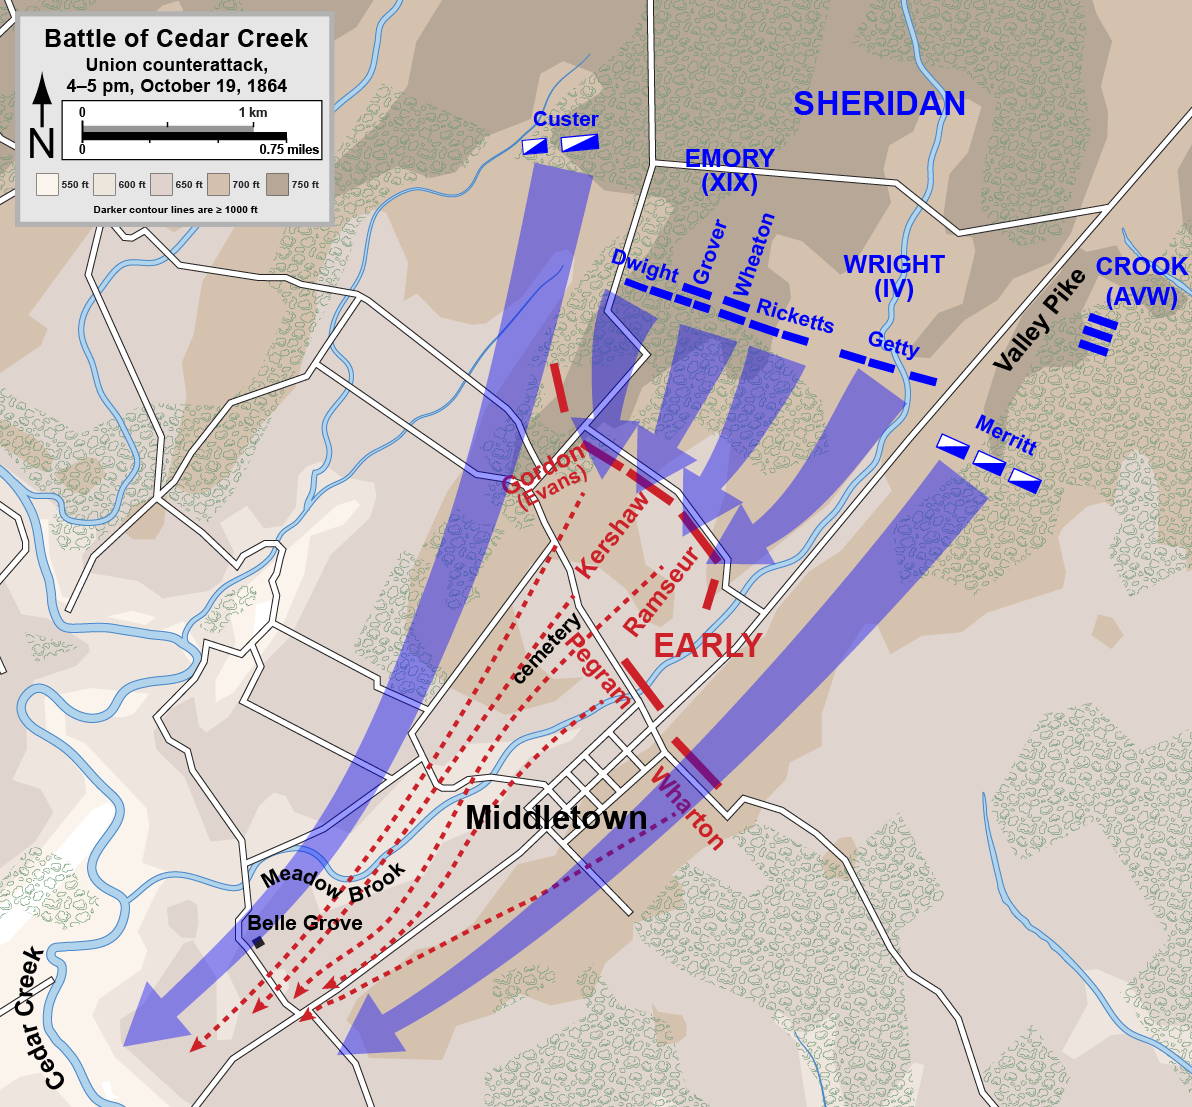
\includegraphics[width=0.5\paperwidth]{../ressources/Cedar_Creek_Union_counterattack}
	};
	\node[draw,item,anchor=south west] at($(current page.south west)+(2.0cm,0.4cm)$) {attaque};
	\node[draw,item,anchor=south east] at($(current page.south east)+(-2.0cm,0.4cm)$) {contre-attaque};
\end{tikzpicture}
\footlineextra{\cite{counterattack_wiki, couterattack_cedar_creek}}
\end{frame}

\begin{frame}{Retraite feinte}
\begin{tikzpicture}[remember picture,overlay]
	\node[anchor=north west,inner sep=0pt] at ($(current page.north west)+(0.1cm,-3cm)$) {
		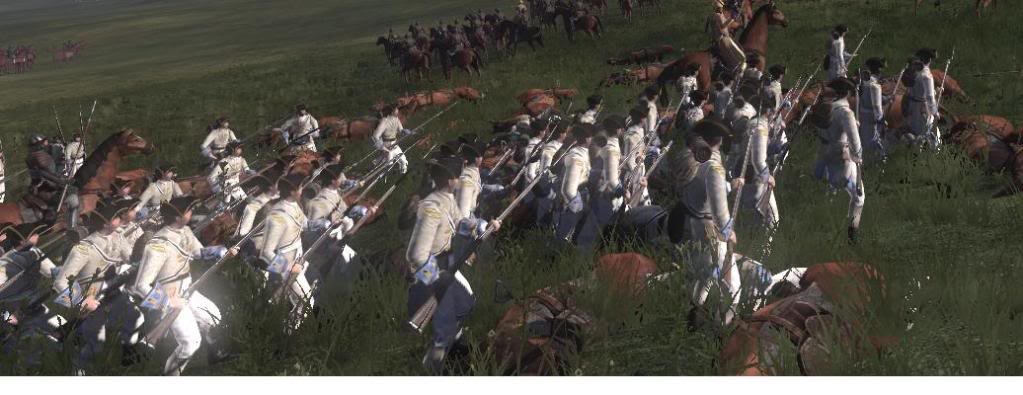
\includegraphics[width=0.98\paperwidth]{../ressources/infantrysquare3}
	};
\end{tikzpicture}
\footlineextra{\cite{mongol_army,feigned_retreat}}
\end{frame}


\begin{frame}{Embuscade}
\begin{tikzpicture}[remember picture,overlay]
	\node[anchor=north east,inner sep=0pt] at ($(current page.north east)+(0.5cm,-0.2cm)$) {
		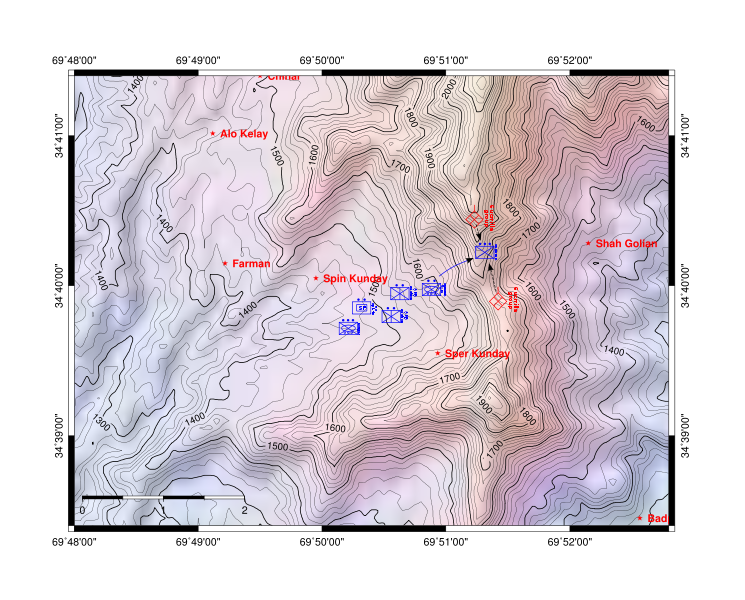
\includegraphics[height=0.8\paperheight]{../ressources/Uzbin_valley_ambush-map}
	};
	\node[anchor=south west,inner sep=0pt] at ($(current page.south west)+(0.1cm,0.45cm)$) {
		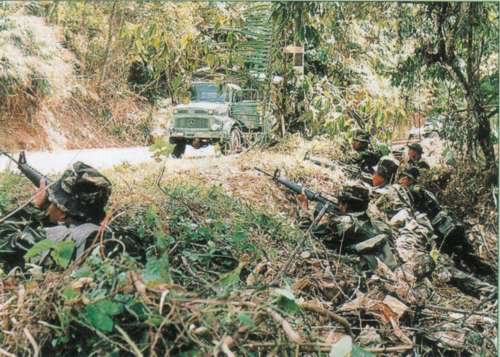
\includegraphics[height=0.3\paperheight]{../ressources/ambush}
	};
\end{tikzpicture}
\footlineextra{\cite{ambush_wiki, uzbin_ambush, ambush_picture}}
\end{frame}

\begin{frame}{Hit and run}
\footlineextra{}
\end{frame}




\section{Applications aux systèmes multi-agents}

\subsection{État de l'art}

\begin{frame}{Enhanced Isaac Neural Simulation Toolkit (EINSTein)}
\framesubtitle{an Artificial-Life Laboratory for Exploring Self-Organized Emergence in Land Combat}
\begin{tikzpicture}[remember picture,overlay]
	\node[draw,item,anchor=north west] at($(current page.north west)+(1.1cm,-5cm)$) {
		Andy Ilachinski
	};
	\node[inner sep=0pt,anchor=north west] at($(current page.north west)+(1.65cm,-5.8cm)$) {
		
\includegraphics[scale=0.5]{../ressources/ilachinski}
	};
	\node[draw,item,anchor=north west] at($(current page.north west)+(1.9cm,-3cm)$) {
		1999
	};
	\node[inner sep=0pt] at (0.6\paperwidth,-0.7cm) {
		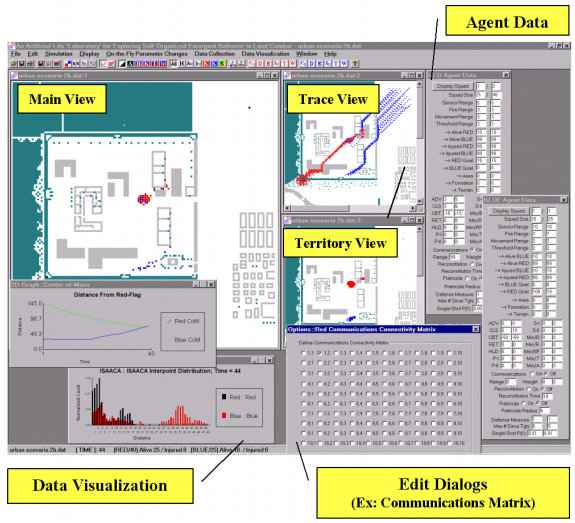
\includegraphics[width=0.7\linewidth]{../ressources/Einstein}
	};
\end{tikzpicture}
\footlineextra{\cite{simu_guerre,ilachinski1994,ilachinski1999}}
\end{frame}

\begin{frame}{Enhanced Isaac Neural Simulation Toolkit (EINSTein)}
\framesubtitle{motivation des agents}
\begin{tikzpicture}[remember picture,overlay]
	\node[inner sep=0pt,anchor=north west] at($(current page.north west)+(0.2cm,-3.3cm)$) {
		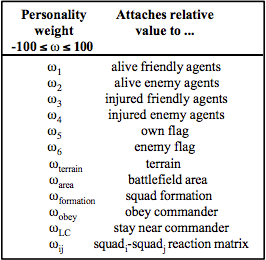
\includegraphics[scale=0.47]{../ressources/einstein_personality_weight}
	};
	\node[inner sep=0pt,anchor=north east] at($(current page.north east)+(-0.2cm,-3cm)$) {
		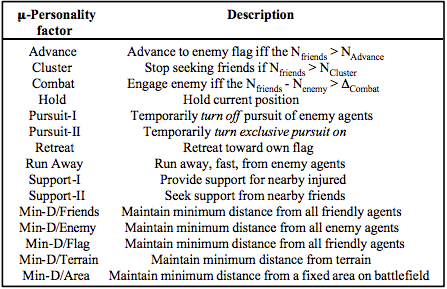
\includegraphics[scale=0.47]{../ressources/einstein_personality_factor}
	};
\end{tikzpicture}
\footlineextra{\cite{ilachinski1994,ilachinski1999}}
\end{frame}

\begin{frame}{Enhanced Isaac Neural Simulation Toolkit (EINSTein)}
\framesubtitle{émergence d'un comportement global}
\begin{tikzpicture}[remember picture,overlay]
	\node[inner sep=0pt,anchor=north west] at($(current page.north west)+(0.2cm,-2cm)$) {
		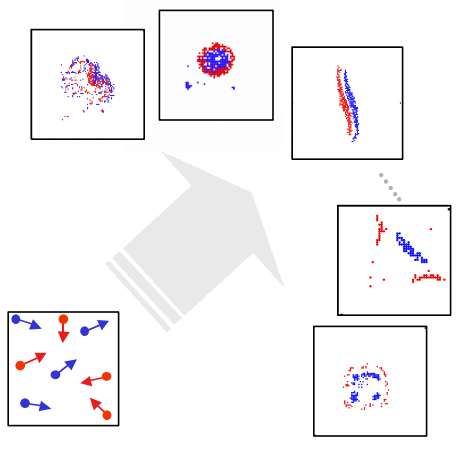
\includegraphics[scale=0.45]{../ressources/einstein_global_behavior}
	};
	\node[draw,item,anchor=south east] at($(current page.south east)+(-1.1cm,6cm)$) {
		formation en pointe
	};
	\node[draw,item,anchor=south east] at($(current page.south east)+(-1.1cm,5cm)$) {
		encerclement
	};
	\node[draw,item,anchor=south east] at($(current page.south east)+(-1.1cm,4cm)$) {
		assault frontal
	};
	\node[draw,item,anchor=south east] at($(current page.south east)+(-1.1cm,3cm)$) {
		prise en tenaille
	};
	\node[draw,item,anchor=south east] at($(current page.south east)+(-1.1cm,2cm)$) {
		guérilla
	};
	\node[draw,item,anchor=south east] at($(current page.south east)+(-1.1cm,1cm)$) {
		\ldots
	};
\end{tikzpicture}
\footlineextra{\cite{ilachinski1994,ilachinski1999}}
\end{frame}

\begin{frame}{Iruba}
\framesubtitle{An Agent-Based Model of the Guerrilla War Process}
\begin{tikzpicture}[remember picture,overlay]
	\node[draw,item,anchor=north west] at($(current page.north west)+(1.4cm,-4.6cm)$) {
		Jim Doran
	};
	\node[inner sep=0pt,anchor=north west] at($(current page.north west)+(0.9cm,-5.4cm)$) {
		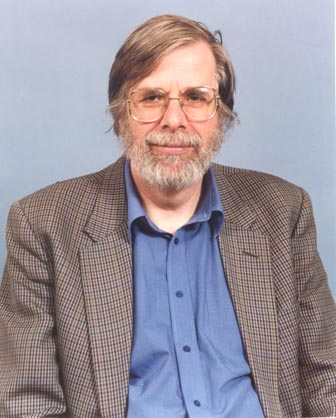
\includegraphics[scale=0.5]{../ressources/doran}
	};
	\node[draw,item,anchor=north west] at($(current page.north west)+(1.8cm,-3cm)$) {
		2005
	};
	\node[inner sep=0pt,anchor=south east] at($(current page.south east)+(-0.1cm,0.4cm)$) {
		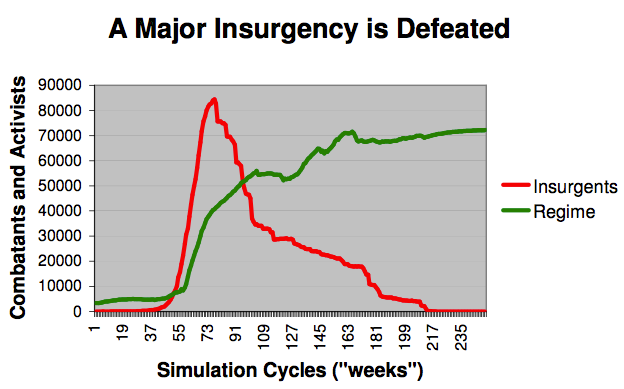
\includegraphics[width=0.5\paperwidth]{../ressources/insurgency}
	};
\end{tikzpicture}
\vspace{-2.8cm}\begin{columns}[t]
	\begin{column}{0.4\paperwidth}
	\end{column}
	\begin{column}[b]{0.5\paperwidth}
            \begin{minipage}[b]{0.5\paperwidth}
		\begin{algorithmic}[1]
		\WHILE{non termination}
			\STATE Attacks and their impact
			\STATE HQ decisions
			\STATE Recruitment
			\STATE Force movement
		\ENDWHILE
		\end{algorithmic}
	\end{minipage}
        \end{column}
\end{columns}
\footlineextra{\cite{doran2005iruba}}
\end{frame}

\begin{frame}{Iruba}
\framesubtitle{Stratégies influentes influentes}
\begin{tikzpicture}[remember picture,overlay]
	\node[draw,item,anchor=north west] at($(current page.north west)+(1.0cm,-3cm)$) {
		initial guerrilla band size
	};
	\node[draw,item,anchor=north west] at($(current page.north west)+(1.4cm,-5cm)$) {
		regime force concentration
	};
	\node[draw,item,anchor=north west] at($(current page.north west)+(8.0cm,-3cm)$) {
		insurgent mobility
	};
	\node[draw,item,anchor=north west] at($(current page.north west)+(6.4cm,-5cm)$) {
		insurgent hyper-mobility
	};
	\node[draw,item,anchor=north west] at($(current page.north west)+(3.8cm,-7cm)$) {
		all-out regime counter attack
	};
\end{tikzpicture}
\footlineextra{\cite{doran2005iruba}}
\end{frame}

\begin{frame}{RPDAgent}
\framesubtitle{Enhanced Military Decision Modeling Using a MultiAgent System Approach}
\begin{tikzpicture}[remember picture,overlay]
	\node[draw,item,anchor=north west] at($(current page.north west)+(0.9cm,-5cm)$) {
		John A. Sokolowski
	};
	\node[inner sep=0pt,anchor=north west] at($(current page.north west)+(1.3cm,-5.8cm)$) {
		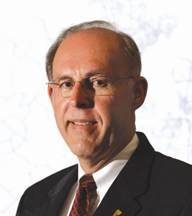
\includegraphics[scale=0.5]{../ressources/john_sokolowski}
	};
	\node[draw,item,anchor=north west] at($(current page.north west)+(1.9cm,-3cm)$) {
		2003
	};
	\node[inner sep=0pt] at (0.6\paperwidth,-0.7cm) {
		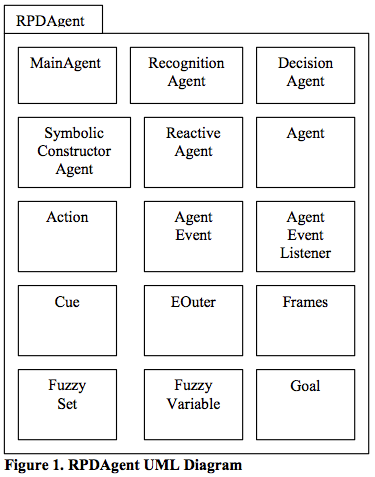
\includegraphics[height=0.7\paperheight]{../ressources/RPDagent_uml}
	};
\end{tikzpicture}
\footlineextra{\cite{sokolowski2003}}
\end{frame}


\subsection{Nos contributions}
\begin{frame}{Une simulation de bataille}
émotions
formations
direct / indirect
\footlineextra{}
\end{frame}


\section{Bibliographie}
\bibliographystyle{plain}
%\bibliographystyle{amsalpha}
\begin{frame}[allowframebreaks]
\frametitle{Bibliographie}
\bibliography{../Bib.bib}
\end{frame}

\end{document}


